\chapter{Experiments and Results}
\label{chapter:chapter05}

The next chapter represents the core experiments of the research. The main purpose of it was to do a benchmark, as a starting point for the comparison between Single Objective Algorithms $SOA$ and Multi Objective algorithms $MOA$. The basis for the experimentation layout was based on the experiments made by H. Ishibuchi, Y. Nojima and T. Doi in \cite{Ishibuchi_single_vs_multiobjective}. \\

The chapter is divided in four different sections, the first section describes the experimental setup. Which are a set of experiments to determine a reference pareto front and the parameters to be used by the algorithms for the rest of the experimentation. whole experimentation process is divided in three different phases: 

\begin{itemize}
    \item The first phase consist in the run of the algorithms without any adjustment using the parameters found in the experimental setup for all the algorithms that applied. 
    \item The second phase is takes into account the results of the first phase of experiments, and the observations and feedback made for about its results. This discusses one of the main issues made by the feedback which remarks weather or not there was made a fair comparison between $SOA$ and $MOA$.
    \item The third phase is the result of a discussion about the tuning of parameters. Using only the best algorithms, chosen by their performance from algorithms from phase one. 
\end{itemize}

\section{Experiments Setup}

The next section discusses a set of experiments that took place before the core experiments could be made. The first subsection shows the experiment made to search for a Reference Pareto Front for the performance comparison. The next subsection shows a experiment for obtaining the base parameters that would be used to have a fair comparison between the algorithms. And the last subsection discusses some of the specific details about each of the individual algorithm implementations.

\subsection{Searching for a Reference Pareto Front}

In order to do a proper comparison, most of the metrics require to have an already established \textbf{Reference Pareto Front}, which in a testing problem would be the \textbf{Real Pareto Front}. \\

In order to establish a \textbf{Pareto Front} for this, the most used algorithm in the literature which is $NSGA-II$ was used with exaggerated parameters to make sure the most of the search space is covered. These parameters consisted of a population of \textbf{20} individuals for \textbf{1000} generations, having \textbf{200} independent runs and selecting the best front for each of the problem sizes. \\

After the experiment, the results of each run were compared with each other, selecting the ones with the lowest \textit{Hypervolume}. These results are shown in Figures~\ref{fig:reference_front_20},\ref{fig:reference_front_200},\ref{fig:reference_front_2000},\ref{fig:reference_front_10001}, for each respective problem. It should be noted in these results, that for the $n=2,000$ and $n=10,0001$ the front shows a concave shape which is characteristic for some minimisation problems. Another important observation is that in the $n=20$ and $n=200$ some of the individuals had the same value for each of their objective functions. This is important because is an indication that a global minima for these problems may exist and could be found using a $SOA$.

\begin{figure}
    \centering
    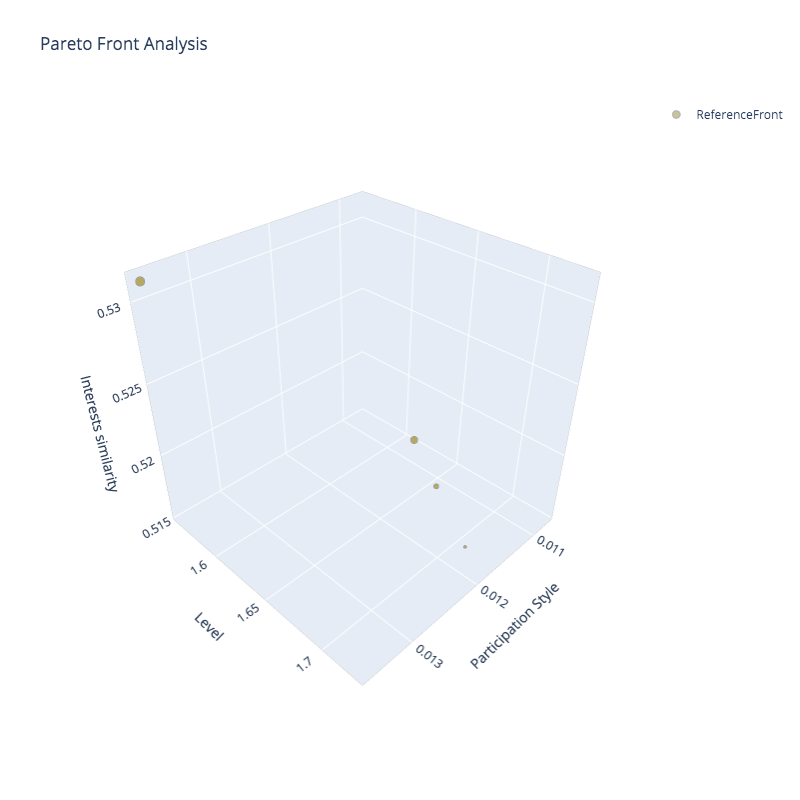
\includegraphics[width=\textwidth]{images/reference_front_20.png}
    \caption{Reference front for the $n=20$ problem. (The evaluation of the $GS$ function is represented by the size of the circles)}
    \label{fig:reference_front_20}
\end{figure}

\begin{figure}
    \centering
    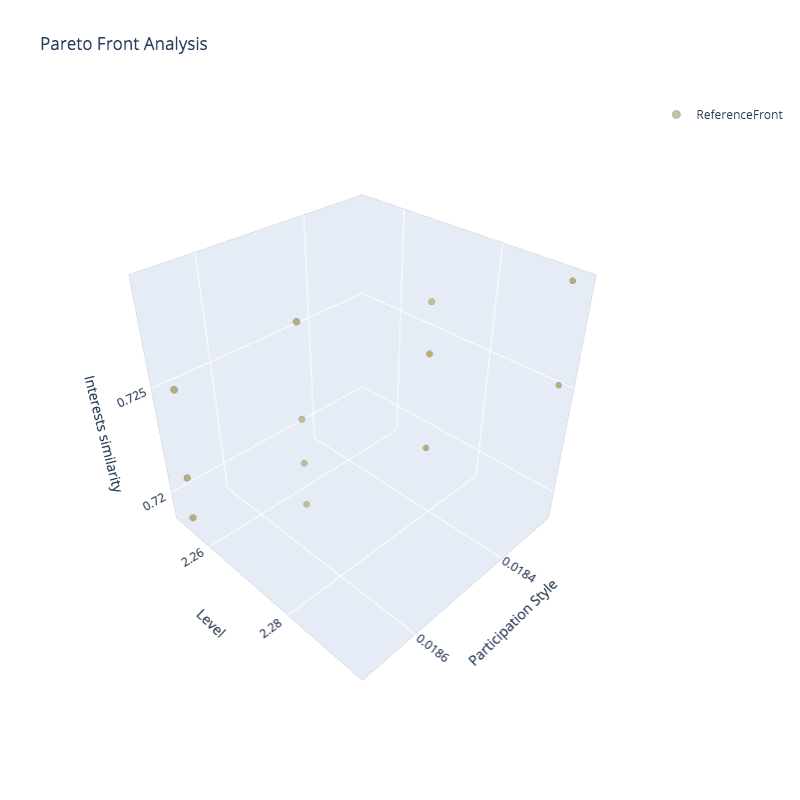
\includegraphics[width=\textwidth]{images/reference_front_200.png}
    \caption{Reference front for the $n=200$ problem. (The evaluation of the $GS$ function is represented by the size of the circles)}
    \label{fig:reference_front_200}
\end{figure}

\begin{figure}
    \centering
    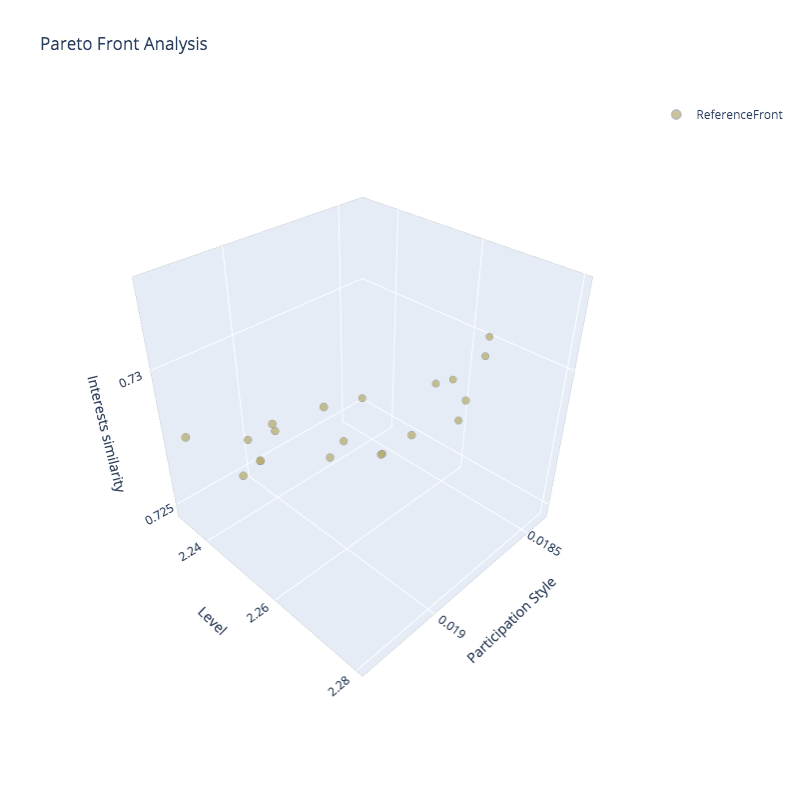
\includegraphics[width=\textwidth]{images/reference_front_2000.png}
    \caption{Reference front for the $n=2,000$ problem. (The evaluation of the $GS$ function is represented by the size of the circles)}
    \label{fig:reference_front_2000}
\end{figure}

\begin{figure}
    \centering
    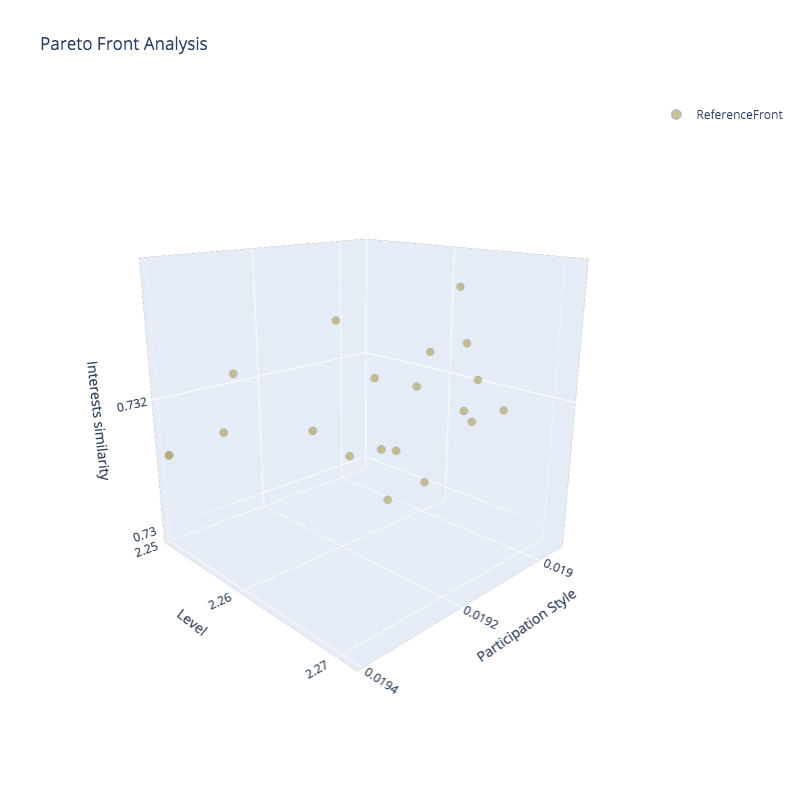
\includegraphics[width=\textwidth]{images/reference_front_10001.png}
    \caption{Reference front for the $n=10,001$ problem. (The evaluation of the $GS$ function is represented by the size of the circles)}
    \label{fig:reference_front_10001}
\end{figure}

\subsection{Searching for Reference Parameters}

Considering that a fair comparison requires a level of complexity similar for each algorithm. The research used the same parameters and the same operators for each of the algorithms. It should be noted that not all the algorithms used all the parameters, only the most shared parameters where considered. This were the number of generations or steps $s$ and the population size. $p$ \\

In this experiment several combinations of these parameters were tested for a $SOA$ and a $MOA$. For the $SOA$ Generational Genetic algorithm $GGA$ was used, whereas for the $MOA$, the algorithm $NSGA-II$ was used. These pairs of parameters $(p,s)$ to be tested were established in a constant scale \textbf{100}, \textbf{150}, \textbf{200}, \textbf{250} and \textbf{300}. For this experiment it were only considered the problem sizes of \textbf{20} and \textbf{200} students. Each pair of parameters was tested for \textbf{50} independent runs\\

It should be noticed that even if both algorithms had a very different optimal set of parameters, another pair could be chosen because it could fairly benefit both types of algorithms. \\

The results are shown in Tables~\ref{table:parameters_soa_20}, \ref{table:parameters_soa_200}, \ref{table:parameters_moa_20}, \ref{table:parameters_moa_200}. Here the best pair and the second best pair is analysed for each of the considered metrics $EP$, $SPREAD$, $GD$, $IGD$, $IGD+$ and also $HV$ for the $MOA$. The main metric to consider was $IGD+$, however the other metrics were also considered here, in case $IGD+$ had little variance between the pairs. After the analysis, it was decided to use a $p=100$ and $s=100$, this is because of the little variance in the $n=200$ problem also, is the most recurrent pair in the results, so it was considered the best across several metrics for $SOA$ and $MOA$ and for the $n=20$ and the $n=200$ problem.

\begin{table}[]
\centering
\resizebox{\textwidth}{!}{
\begin{tabular}{lcccc}
\hline
    & Best $(p,s)$     & Best Value & Second Best $(p,s)$ & Second Best Value  \\
    \hline
    EP Mean and STD            & 150,250  & $8.77e + 00_{3.5e+00}$ & 100,150 & $8.98e + 00_{3.9e+00}$ \\
    EP Med and Inter Range     & 250,250  & $9.45e + 00_{2.9e+00}$ & 300,150 & $9.46e + 00_{3.4e+00}$ \\
    SPREAD Mean and STD        & 100,100  & $1.00e + 00_{0.0e+00}$ & 150,100 & $1.00e + 00_{0.0e+00}$ \\
    SPREAD Med and Inter Range & 100,100  & $1.00e + 00_{0.0e+00}$ & 150,100 & $1.00e + 00_{0.0e+00}$ \\
    GD Mean and STD            & 150,250  & $9.27e + 00_{3.9e+00}$ & 250,250 & $9.29e + 00_{3.6e+00}$ \\
    GD Med and Inter Range     & 250,300  & $9.84e + 00_{3.7e+00}$ & 250,250 & $9.92e + 00_{3.6e+00}$ \\
    IGD Mean and STD           & 150,250  & $2.25e + 00_{9.0e−01}$ & 250,250 & $2.25e + 00_{8.3e−01}$ \\
    IGD Med and Inter Range    & 250,300  & $2.40e + 00_{8.3e−01}$ & 250,250 & $2.42e + 00_{8.8e−01}$ \\
    IGD+ Mean and STD          & 150,250  & $9.80e + 00_{4.3e+00}$ & 250,250 & $9.93e + 00_{3.9e+00}$ \\
    IGD+ Med and Inter Range   & 250,300  & $1.07e + 01_{3.7e+00}$ & 250,250 & $1.08e + 01_{3.9e+00}$ \\
    \hline 
    \end{tabular}
}
\caption{The results of the parameters experiment of $n=20$ for $SOA$, by combinations of a population size $p$ and a number of steps or generations $s$}
\label{table:parameters_soa_20}
\end{table}

\begin{table}[]
\centering
\resizebox{\textwidth}{!}{
    \begin{tabular}{lcccc}
    \hline
    & Best $(p,s)$ & Best Value & Second Best $(p,s)$ & Second Best Value   \\
    \hline
    EP Mean and STD            & 100,100 & $3.97e + 01_{5.6e+00}$  & 200,150  & $3.99e + 01_{5.4e+00}$   \\
    EP Med and Inter Range     & 200,150 & $3.94e + 01_{7.6e+00}$  & 250, 300 & $3.96e + 01_{8.0e+00}$   \\
    SPREAD Mean and STD        & 100,100 & $1.00e + 00_{0.0e+00}$  & 150,100  & $1.00e + 00_{0.0e+00}$   \\
    SPREAD Med and Inter Range & 100,100 & $1.00e + 00_{0.0e+00}$  & 150,100  & $1.00e + 00_{0.0e+00}$   \\
    GD Mean and STD            & 100,100 & $4.04e + 01_{5.8e+00}$  & 200,150  & $4.05e + 01_{5.6e+00}$   \\
    GD Med and Inter Range     & 200,150 & $4.02e + 01_{7.8e+00}$  & 250,300  & $4.03e + 01_{7.9e+00}$   \\
    IGD Mean and STD           & 100,100 & $9.16e + 00_{1.3e+00}$  & 200,150  & $9.18e + 00_{1.2e+00}$   \\
    IGD Med and Inter Range    & 200,150 & $9.12e + 00_{1.7e+00}$  & 250,300  & $9.15e + 00_{1.7e+00}$   \\
    IGD+ Mean and STD          & 100,100 & $4.00e + 01_{5.9e+00}$  & 200,150  & $4.01e + 01_{5.7e+00}$   \\
    IGD+ Med and Inter Range   & 200,150 & $3.96e + 01_{7.9e+00}$  & 250,300  & $3.98e + 01_{8.4e+00}$   \\
    \hline
    \end{tabular}
}
\caption{The results of the parameters experiment of $n=200$ for $SOA$, by combinations of a population size $p$ and a number of steps or generations $s$}
\label{table:parameters_soa_200}
\end{table}

\begin{table}[]
\centering
\resizebox{\textwidth}{!}{%
\begin{tabular}{lcccc}
\hline
                           & Best $(p,s)$   & Best Value             & Second Best $(p,s)$ & Second Best Value  \\
\hline
EP Mean and STD            & 100,300 & $2.83e + 00_{2.2e+00}$ & 300,100 & $3.08e + 00_{2.4e+00}$ \\
EP Med and Inter Range     & 200,300 & $1.63e + 00_{4.3e+00}$ & 100,300 & $1.69e + 00_{4.0e+00}$ \\
SPREAD Mean and STD        & 100,100 & $1.00e + 00_{0.0e+00}$ & 150,100 & $1.00e + 00_{0.0e+00}$ \\
SPREAD Med and Inter Range & 100,100 & $1.00e + 00_{0.0e+01}$ & 150,101 & $1.00e + 00_{0.0e+01}$ \\
GD Mean and STD            & 100,300 & $1.44e - 01_{1.4e-01}$ & 300,300 & $1.79e - 01_{1.8e-01}$ \\
GD Med and Inter Range     & 100,300 & $8.18e - 02_{2.4e-01}$ & 200,300 & $8.97e - 02_{2.9e-01}$ \\
IGD Mean and STD           & 100,300 & $7.14e - 01_{5.4e-01}$ & 300,100 & $7.51e - 01_{5.9e-01}$ \\
IGD Med and Inter Range    & 100,300 & $4.14e - 01_{8.9e-01}$ & 300,100 & $4.14e - 01_{9.8e-01}$ \\
IGD+ Mean and STD          & 100,300 & $2.89e + 00_{2.5e+00}$ & 300,100 & $3.19e + 00_{2.7e+00}$ \\
IGD+ Med and Inter Range   & 200,300 & $1.48e + 00_{4.5e+00}$ & 100,250 & $1.64e + 00_{7.1e+00}$ \\
HV Mean and STD            & 150,150 & $3.66e + 01_{6.4e+01}$ & 100,100 & $3.51e + 01_{5.9e+01}$ \\
HV Med and Inter Range     & 200,100 & $9.78e + 00_{4.5e+01}$ & 300,200 & $6.20e + 00_{3.4e+01}$ \\
\hline
\end{tabular}
}
\caption{The results of the parameters experiment of $n=20$ for $MOA$, by combinations of a population size $p$ and a number of steps or generations $s$}
\label{table:parameters_moa_20}
\end{table}

\begin{table}[]
\centering
\resizebox{\textwidth}{!}{%
\begin{tabular}{lcccc}
\hline
                           & Best $(p,s)$   & Best Value             & Second Best $(p,s)$ & Second Best Value        \\
\hline
EP Mean and STD            & 100,100 & $5.42e + 00_{2.3e+00}$ & 100,200     & $6.37e + 00_{3.3e+00}$ \\
EP Med and Inter Range     & 100,100 & $5.32e + 00_{2.8e+00}$ & 100,200     & $5.64e + 00_{5.3e+00}$ \\
SPREAD Mean and STD        & 250,300 & $1.00e + 00_{0.0e+00}$ & 300,300     & $1.00e + 00_{0.0e+00}$ \\
SPREAD Med and Inter Range & 150,100 & $1.00e + 00_{0.0e+00}$ & 200,100     & $1.00e + 00_{0.0e+00}$ \\
GD Mean and STD            & 100,200 & $4.59e - 01_{2.4e-01}$ & 100,300     & $5.08e - 01_{2.3e-01}$ \\
GD Med and Inter Range     & 100,200 & $4.08e - 01_{3.5e-01}$ & 100,150     & $5.03e - 01_{5.1e-01}$ \\
IGD Mean and STD           & 100,100 & $1.24e + 00_{5.0e-01}$ & 100,150     & $1.50e + 00_{7.4e-01}$ \\
IGD Med and Inter Range    & 100,100 & $1.18e + 00_{6.2e-01}$ & 100,200     & $1.34e + 00_{1.2e+00}$ \\
IGD+ Mean and STD          & 100,100 & $5.33e + 00_{2.3e+00}$ & 100,150     & $6.37e + 00_{3.5e+00}$ \\
IGD+ Med and Inter Range   & 100,100 & $5.21e + 00_{3.0e+00}$ & 100,200     & $5.47e + 00_{5.2e+00}$ \\
HV Mean and STD            & 300,250 & $4.49e + 02_{6.4e+02}$ & 300,200     & $4.40e + 02_{5.7e+02}$ \\
HV Med and Inter Range     & 200,250 & $2.39e + 02_{3.9e+02}$ & 300,150     & $2.07e + 02_{4.2e+02}$ \\
\hline
\end{tabular}%
}
\caption{The results of the parameters experiment of $n=200$ for $MOA$, by combinations of a population size $p$ and a number of steps or generations $s$}
\label{table:parameters_moa_200}
\end{table}

\subsection{Details per implementation}

Since this part of the research is only considered as a starting point, the default values and additional configurations for all the algorithms were left for each experiment. Here the descriptions for all the algorithms is given with each of their specific implementations for the problem. As previously noted, all the implementations were already included in the \textbf{jMetal} and \textbf{JAMES} frameworks, and the only extra functions created were the mutation and crossover operators and the problem and solution definitions.

\subsubsection{Single-Objective Algorithms}

A disadvantage found in the experiments of \ref{chapter:chapter04} were that for the $SOA$, the ranges of each of the objective functions varied considerably, which added more weight for the higher evaluation results. To address this issue an a posteriori normalisation of the parameters was established shown in Table~\ref{table:normalization_parameters} using the Equation~\ref{eq:normalization_equation}. \\

The full details of each of the implementations can be seen in Table~\ref{table:soa_details_jmetal} for the algorithms used present in the jMetal framework, and Table~\ref{table:soa_details_james} for the algorithms used present in the James framework.

\begin{equation}
    v_{norm} = \frac{v- v_{min}}{v_{max} - v_{vmin}} 
    \label{eq:normalization_equation}
\end{equation}

\begin{table}[]
    \begin{tabular}{lll}
    \hline
    Objective function & Minimum value $v_{min}$ & Maximum value $v_{max}$ \\
    \hline
    Group Size Function                  & 0.5                     & 1.5                     \\
    Participation Style Function         & 0.001666                & 1.0                     \\
    Level Function                       & 0.0                     & 2.82843                 \\
    Interests Cosine Similarity Function & 0.0                     & 1.0                     \\
    \hline
    \end{tabular}
    \caption{The $v_{min}$ and $v_{max}$ values for each objective function used in the normalisation}
    \label{table:normalization_parameters}
\end{table}

\begin{table}[]
    \begin{tabular}{p{0.15\textwidth}p{0.15\textwidth}p{0.30\textwidth}p{0.24\textwidth}p{0.10\textwidth}}
    \hline
    Denomination  & Full name & Details & Additional Parameters
    \\
    \hline
    $GGA$ & Genetic Generational Algorithm & Is an implementation of the Genetic Algorithm in which all the solutions are replaced in each of the generations. & n/a \\ \\
    $GSA$ & Genetic Steady Algorithm & Is an implementation of the Genetic Algorithm in which a single solution is added and another one is eliminated in each generation & n/a \\ \\
    $Elitist$ & Elitist Algorithm $(\mu + \lambda)$ & Randomly selects a parent form the set of $\mu$ individuals from both the parents and offspring of the last generation, the parent is then mutated and generates $\lambda$ offsprings. & $\mu = 1$; $\lambda = pop (100)$ \\ \\
    $Non - Elitist$ & Non-Elitist Algorithm $(\mu,\lambda)$ & Randomly selects a parent form the set of $\mu$ individuals from both the parents and offspring of the last generation, and the parent is then mutated and generates $\lambda$ offsprings  & $\lambda = pop (100)$ \\ \\
    $LS$ & Local Search (Steepest Descent/Hill Climbing) & The implementation found in the framework jMetal, was the one used as a middle step procedure for other algorithms like $ABYSS$. it makes use of a Dominance comparator & $\epsilon = 0$ \\ \\
    $RS$ & Random Search & n/a & n/a  \\ \\
    \hline
    \end{tabular}
    \caption{Specific details of the Single-Objective Algorithms Implementations based on the jMetal Framework}
    \label{table:soa_details_jmetal}
\end{table}

\begin{table}[]
    \begin{tabular}{p{0.15\textwidth}p{0.15\textwidth}p{0.30\textwidth}p{0.24\textwidth}p{0.10\textwidth}}
    \hline
    Denomination  & Full name & Details & Additional Parameters 
    \\
    \hline
    $RD$ & Random Descent & The neighbourhood is considered as a mutation step, so all the possible mutations are considered in each step. & n/a \\ \\
    $PT$ & Parallel Tempering (Replica Exchange Monte Carlo) & Similar to Simulated Annealing this algorithm uses a max temperature and a low temperature, also running parallel replicas of Metropolis search.& $temp_{min} = 1 * 1e^{-8}$;$temp_{max} = 1 * 0.6$; $steps_{max} = 100$; $replicas = 2$ \\ \\
    \hline
    \end{tabular}
    \caption{Specific details of the Single-Objective Algorithms Implementations based on the James Framework}
    \label{table:soa_details_james}
\end{table}

\subsubsection{Multi-Objective algorithms}

The details and specific parameters for the Multi-Objective algorithms can be seen in Table~\ref{table:moa_details}, in this case, all the algorithms implementations belong to the jMetal framework. It should also be noted that as a general parameter a $Binary Tourmament Selection$ and a $Ranking and Crowding Distance Comparator$ was used for all these algorithms.

\begin{table}[]
    \begin{tabular}{p{0.15\textwidth}p{0.15\textwidth}p{0.30\textwidth}p{0.30\textwidth}}
    \hline
    Denomination  & Full Name & Details & Additional parameters \\
    \hline
    $ESPEA$         & Electrostatic Potential Energy Evolutionary Algorithm  & Since no scalarized preference is specified, uniform preferences are assumed
    Uses a Worst in Archive Replacement Strategy. 
    Where Among all eligible archive members that can be replaced the one exhibiting the largest energy contribution is replaced. & Replacement Strategy: Worst in Archive \\ \\
    $MOMBI2$        & Many Objective Metaheuristic Based on the R2 Indicator & Requires a number of weights equal to the population size. These weights were selected according to the population size using the Simplex-Lattice Design method & Vector of weights, using Simple-Lattice Design method; According to the population size. \\ \\
    $NSGA-II$       & Non-dominated Sorting Genetic Algorithm               & n/a \\ \\
    $RS$           & Random Search                                          & n/a  & n/a \\ \\ 
    $SPEA2$        & Strength Pareto Evolutionary Algorithm                 & n/a  & n/a \\ \\
    \hline                                                                                                                 
    \end{tabular}
    \caption{Specific details of the Multi-Objective Algorithms Implementations}
    \label{table:moa_details}
\end{table}

\section{First Phase}

The first phase of experiments run all the algorithms with the established operators and parameters defined in the previous section, and using the found Pareto Front approximation for the metrics. Then for the results, the first set of $SOA$ were compared with each other. This is also the case for $MOA$, finally the best algorithm for each of these two categories was taken and compared with each other. Each algorithm was tested with \textbf{30} independent runs.

\subsection{Comparison between Single-Objective Algorithms}

\begin{figure}
    \centering
    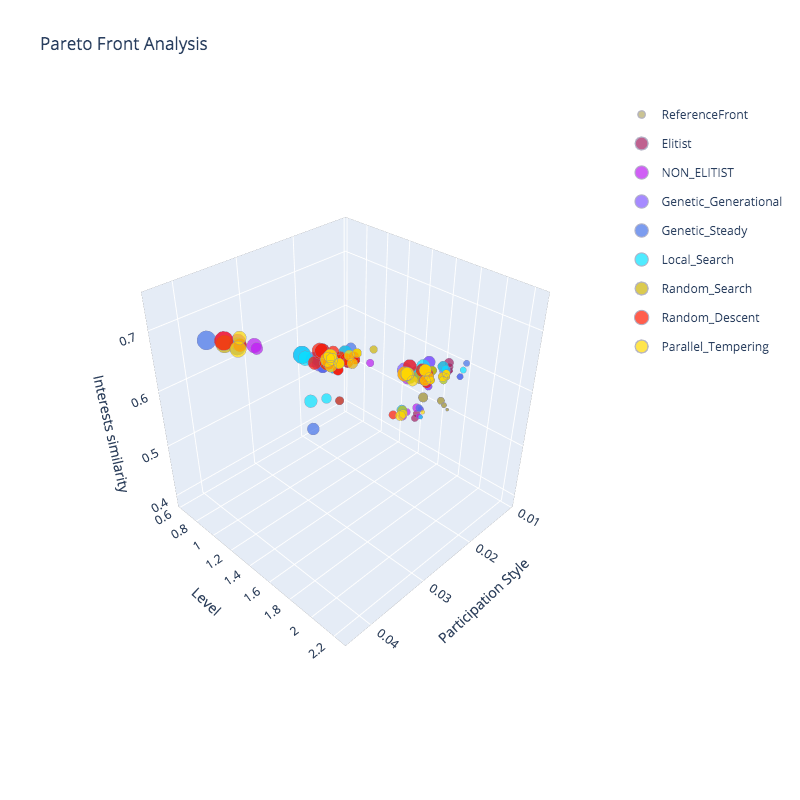
\includegraphics[width=\textwidth]{images/3d_soa_20.png}
    \caption{Caption}
    \label{fig:my_label}
\end{figure}

\begin{figure}
    \centering
    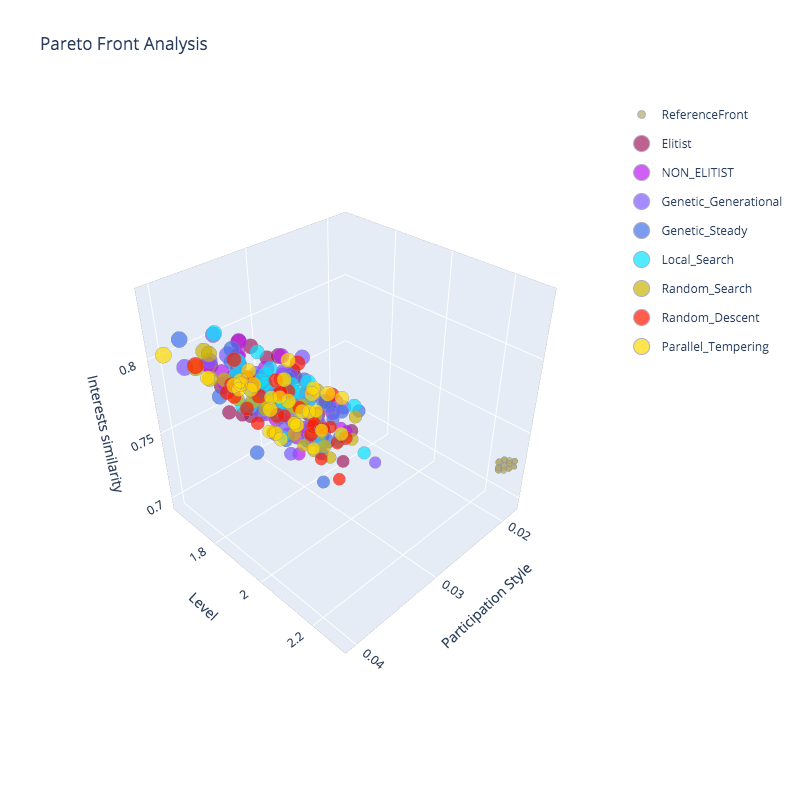
\includegraphics[width=\textwidth]{images/3d_soa_200.png}
    \caption{Caption}
    \label{fig:my_label}
\end{figure}

\begin{figure}
    \centering
    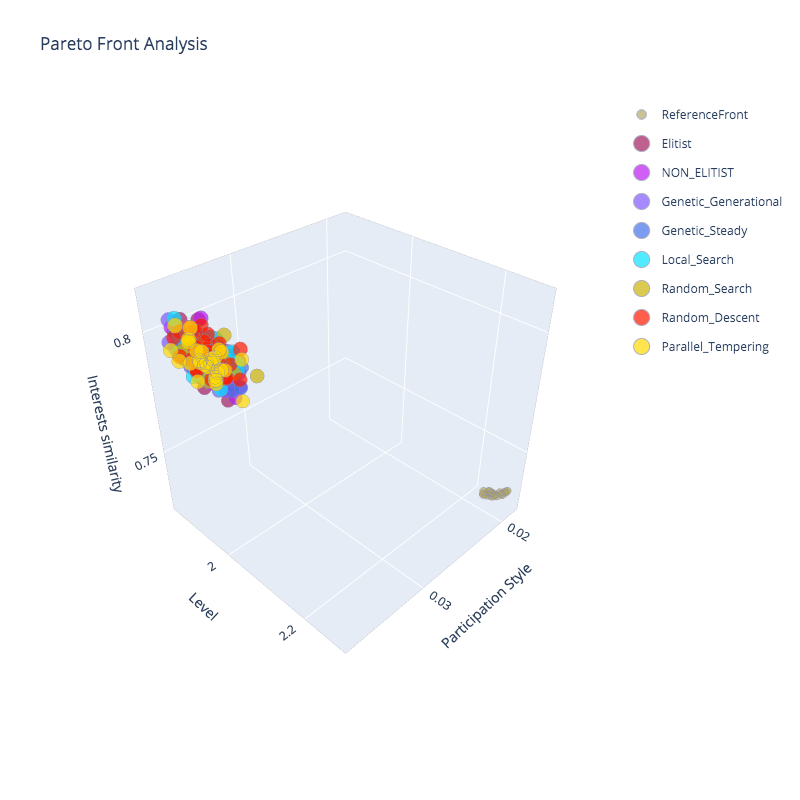
\includegraphics[width=\textwidth]{images/3d_soa_2000.png}
    \caption{Caption}
    \label{fig:my_label}
\end{figure}

\begin{figure}
    \centering
    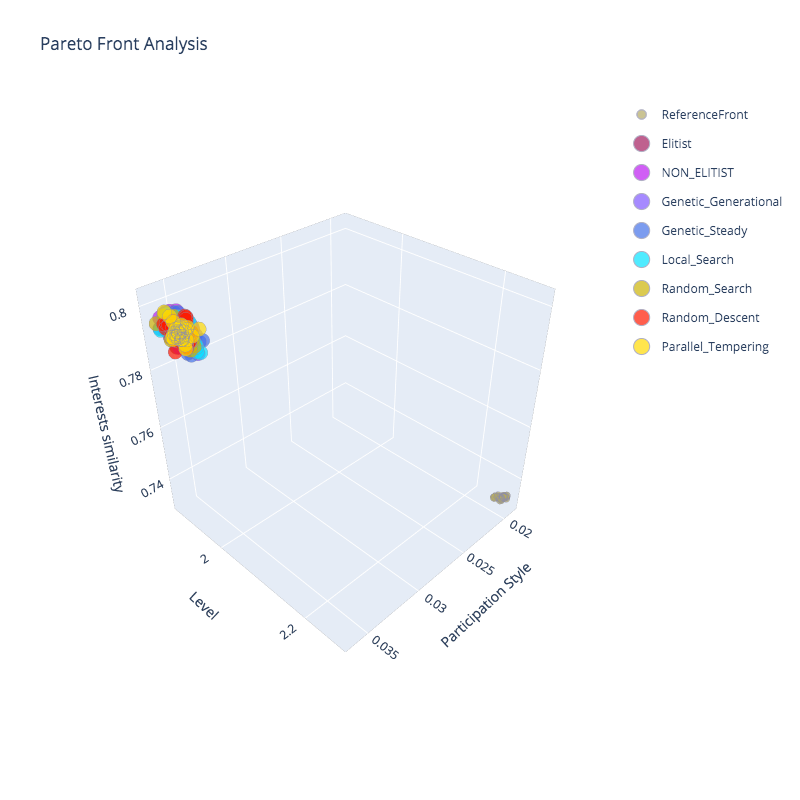
\includegraphics[width=\textwidth]{images/3d_soa_10001.png}
    \caption{Caption}
    \label{fig:my_label}
\end{figure}

\begin{figure}
    \centering
    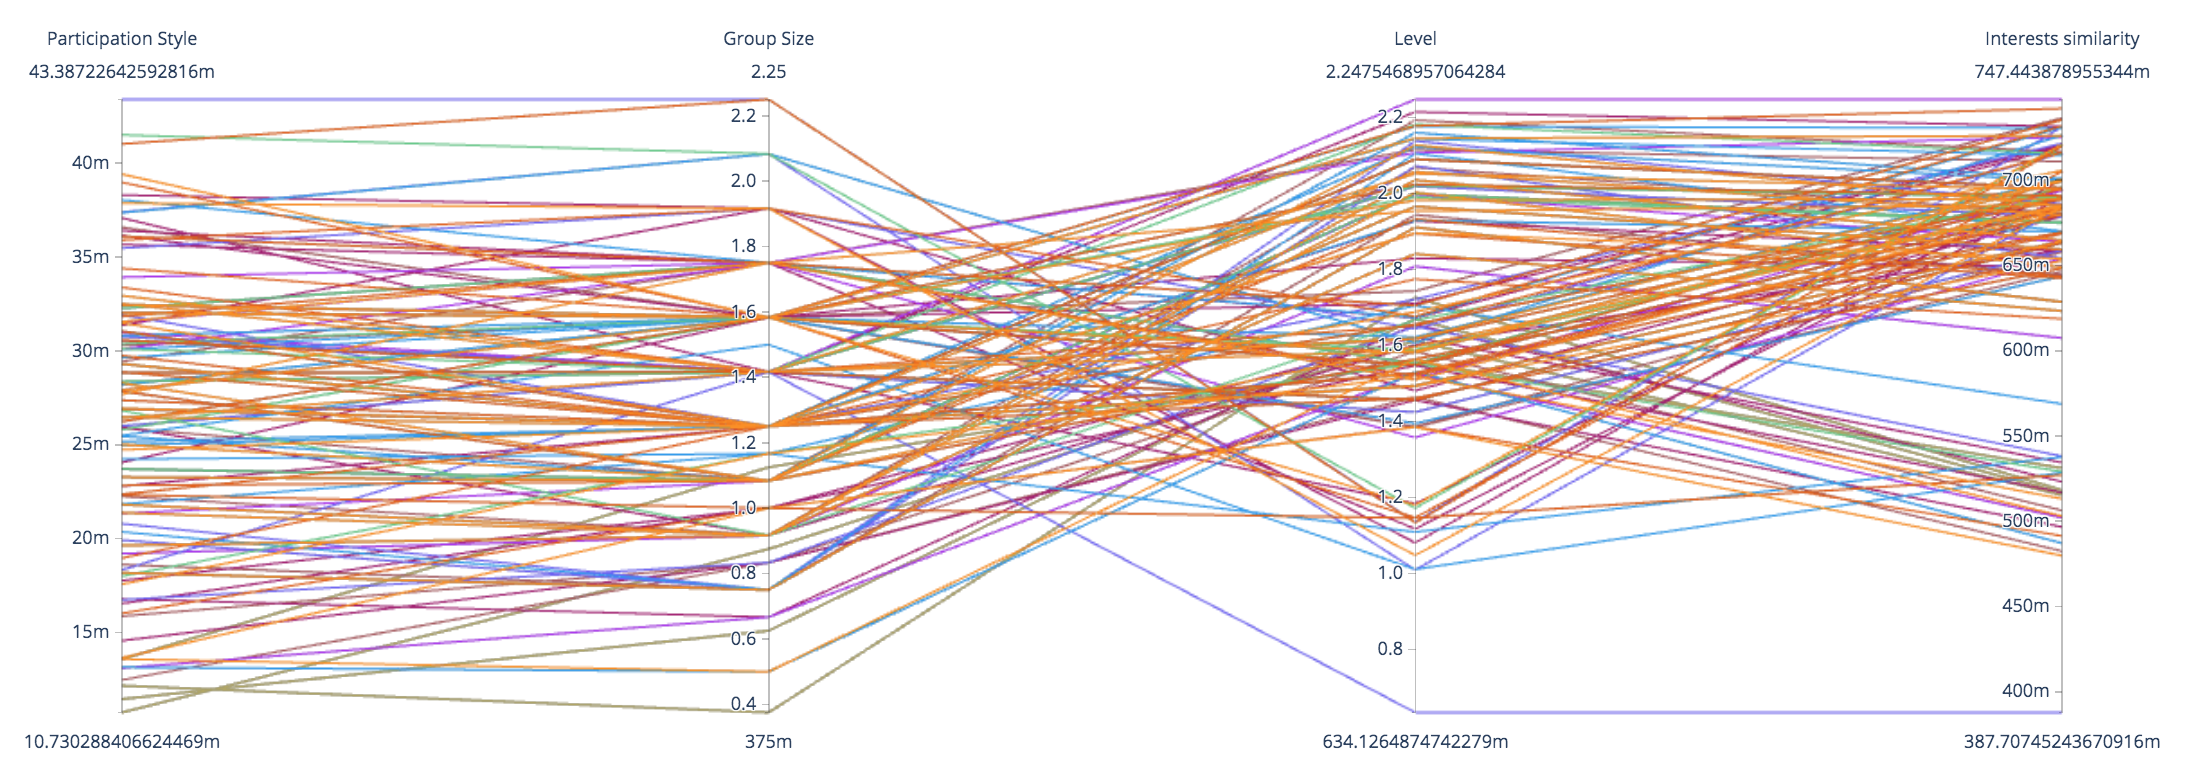
\includegraphics[width=\textwidth]{images/para_soa_20.png}
    \caption{Caption}
    \label{fig:my_label}
\end{figure}

\begin{figure}
    \centering
    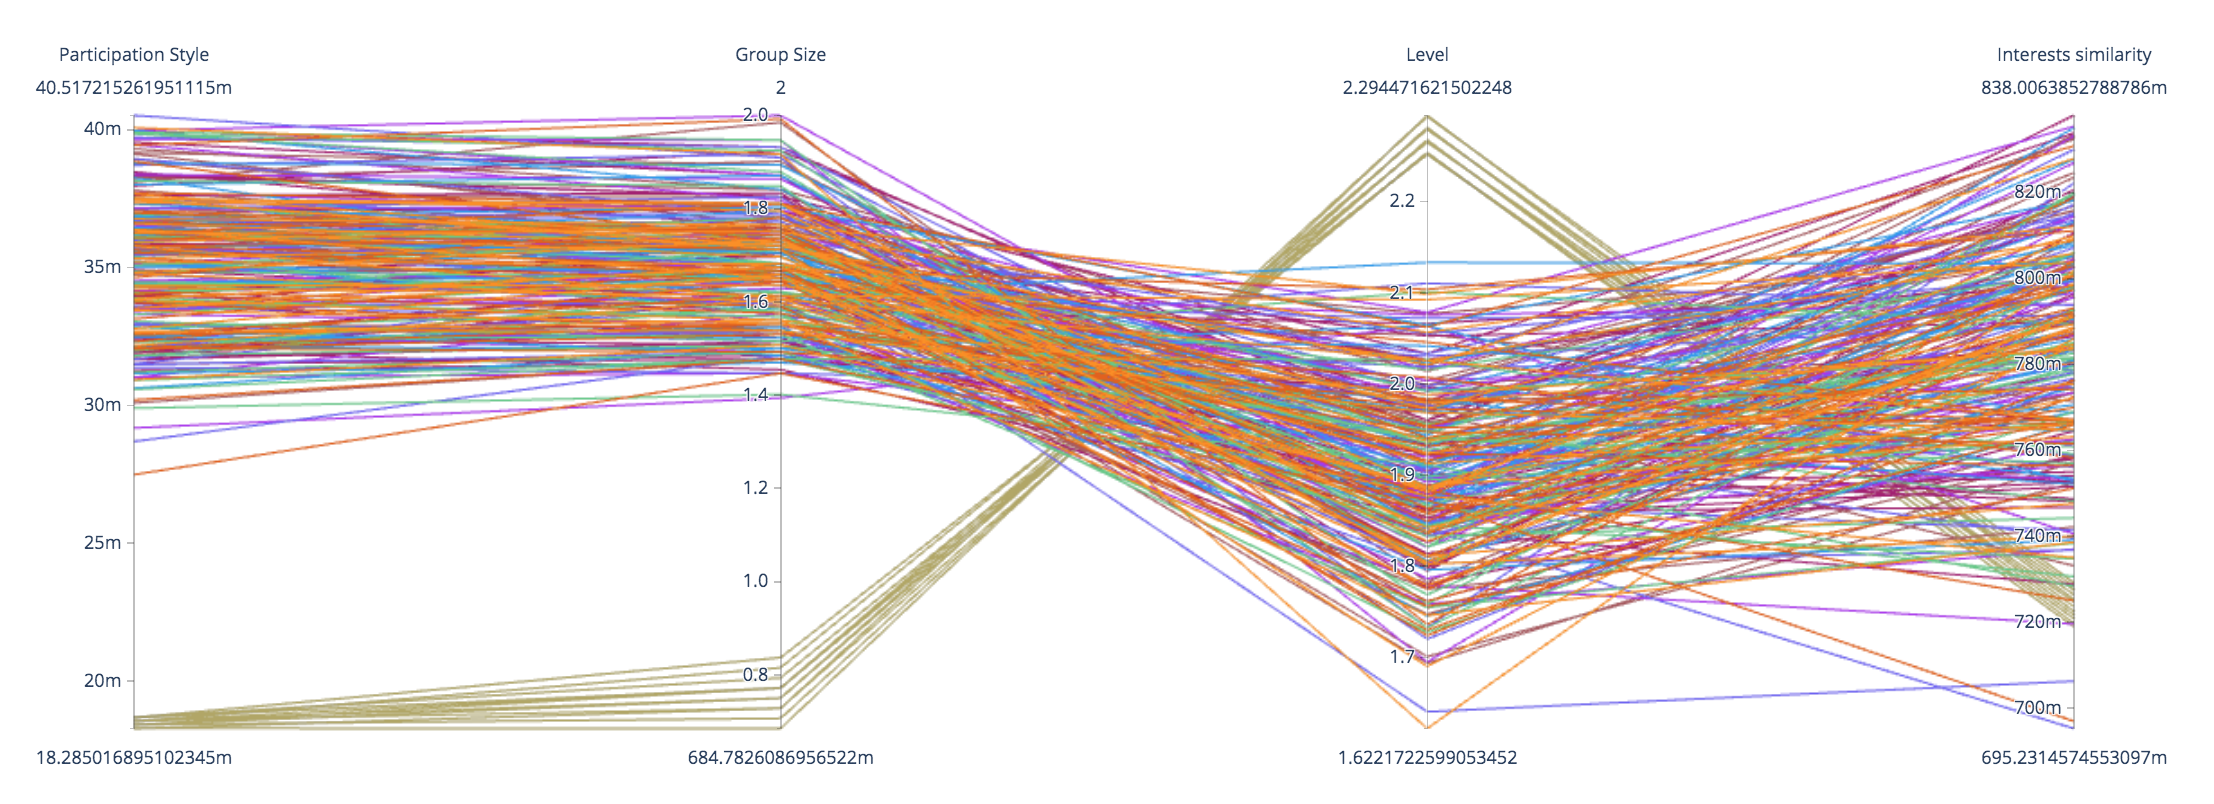
\includegraphics[width=\textwidth]{images/para_soa_200.png}
    \caption{Caption}
    \label{fig:my_label}
\end{figure}

\begin{figure}
    \centering
    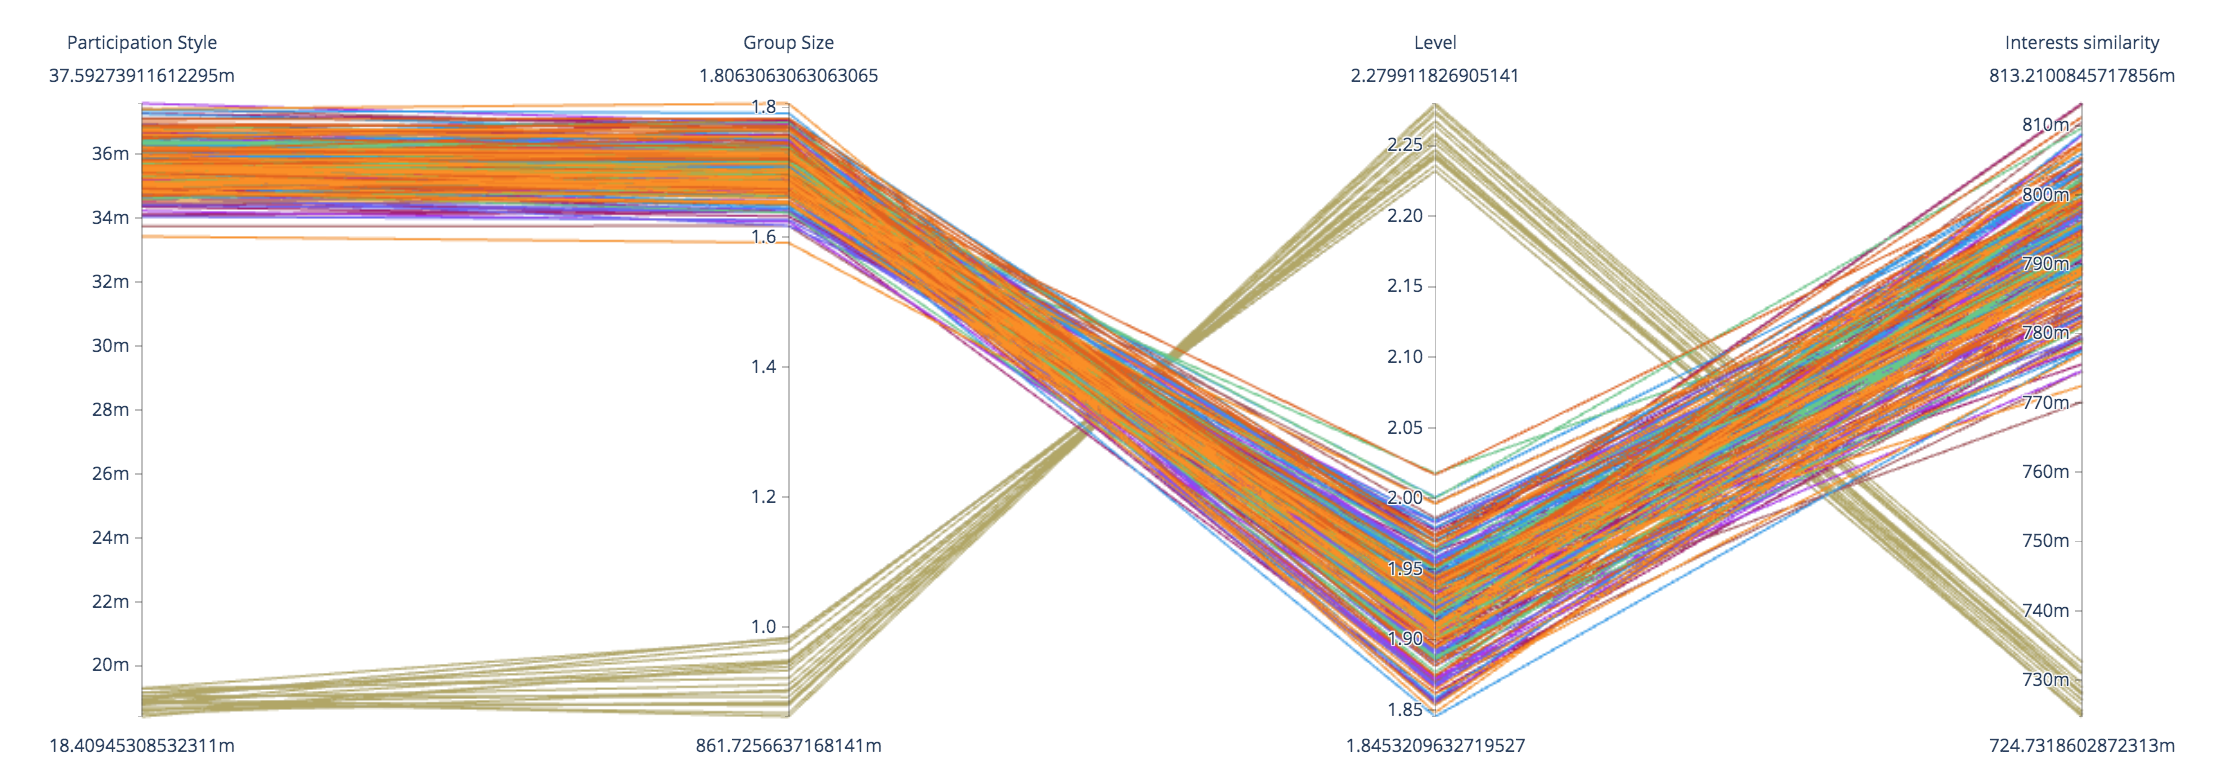
\includegraphics[width=\textwidth]{images/para_soa_2000.png}
    \caption{Caption}
    \label{fig:my_label}
\end{figure}

\begin{figure}
    \centering
    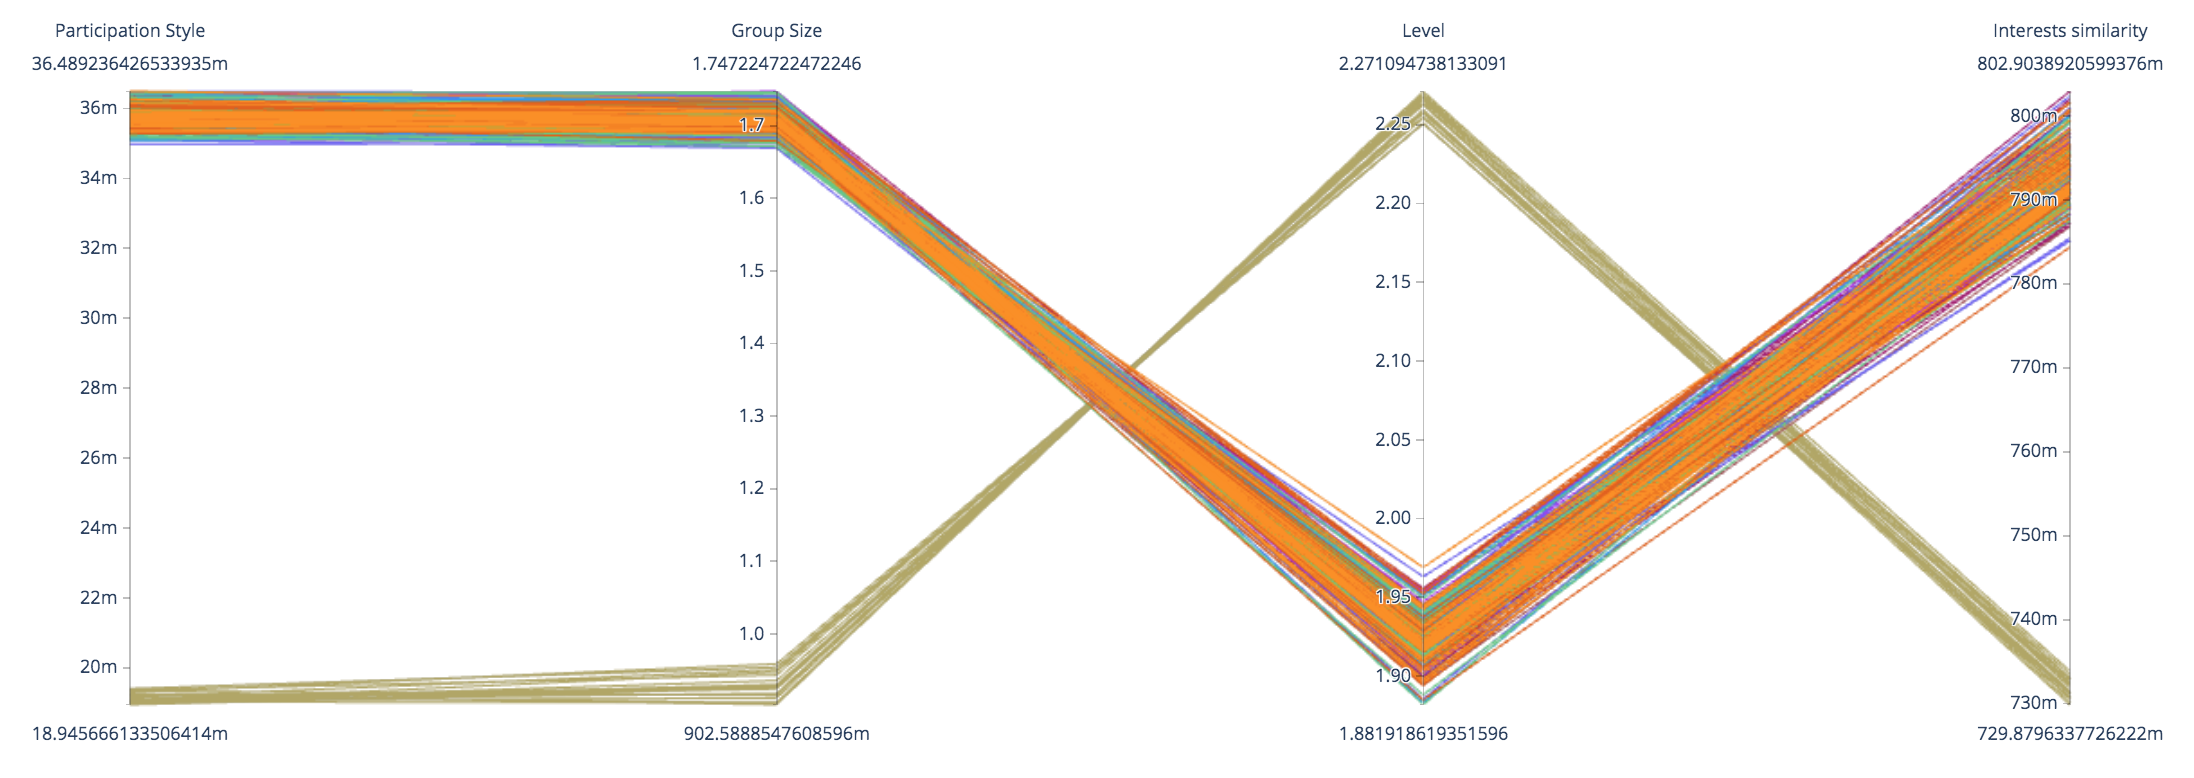
\includegraphics[width=\textwidth]{images/para_soa_10001.png}
    \caption{Caption}
    \label{fig:my_label}
\end{figure}

% Please add the following required packages to your document preamble:
% \usepackage{booktabs}
% \usepackage{graphicx}
\begin{table}[]
\centering
\resizebox{\textwidth}{!}{%
\begin{tabular}{@{}lllll@{}}
\hline
                     & Grouping\_Problem\_20                     & Grouping\_Problem\_200                    & Grouping\_Problem\_2000                   & Grouping\_Problem\_10001                  \\ 
\hline
ESPEA                & $  5.45e+00_{ 3.0e+00}$                   & \cellcolor{gray25}$  3.62e+00_{ 2.3e+00}$ & $  1.51e+00_{ 1.1e-01}$                   & $  2.49e+00_{ 1.2e-01}$                   \\
MOMBI                & \cellcolor{gray25}$  4.01e+00_{ 2.5e+00}$ & $  9.36e+00_{ 4.2e+00}$                   & $  2.19e+00_{ 2.8e-01}$                   & $  2.97e+00_{ 2.1e-01}$                   \\
NSGAII               & $  4.76e+00_{ 2.8e+00}$                   & $  5.29e+00_{ 2.6e+00}$                   & \cellcolor{gray25}$  1.49e+00_{ 1.6e-01}$ & \cellcolor{gray25}$  2.48e+00_{ 9.7e-02}$ \\
RS                   & \cellcolor{gray95}$  0.00e+00_{ 0.0e+00}$ & \cellcolor{gray95}$  1.98e-01_{ 1.1e-01}$ & \cellcolor{gray95}$  1.14e+00_{ 6.4e-02}$ & \cellcolor{gray95}$  2.15e+00_{ 5.8e-02}$ \\
SPEA2                & $  5.47e+00_{ 3.4e+00}$                   & $  5.00e+00_{ 3.1e+00}$                   & $  1.68e+00_{ 1.6e-01}$                   & $  2.63e+00_{ 1.5e-01}$                   \\
Random_Descent       & $  1.02e+01_{ 2.5e+00}$                   & $  4.08e+01_{ 6.2e+00}$                   & $  1.98e+01_{ 7.9e-01}$                   & $  3.74e+01_{ 6.5e-01}$                   \\
Parallel_Tempering   & $  9.37e+00_{ 3.2e+00}$                   & $  4.20e+01_{ 5.0e+00}$                   & $  1.95e+01_{ 9.2e-01}$                   & $  3.74e+01_{ 5.4e-01}$                   \\
Random_Search        & $  9.84e+00_{ 2.0e+00}$                   & $  4.01e+01_{ 6.6e+00}$                   & $  1.97e+01_{ 6.0e-01}$                   & $  3.74e+01_{ 7.7e-01}$                   \\
Local_Search         & $  9.70e+00_{ 3.1e+00}$                   & $  4.19e+01_{ 5.5e+00}$                   & $  1.99e+01_{ 7.9e-01}$                   & $  3.73e+01_{ 7.5e-01}$                   \\
Genetic_Steady       & $  1.00e+01_{ 2.8e+00}$                   & $  4.17e+01_{ 7.0e+00}$                   & $  1.96e+01_{ 7.5e-01}$                   & $  3.75e+01_{ 8.6e-01}$                   \\
Genetic_Generational & $  9.98e+00_{ 2.7e+00}$                   & $  4.19e+01_{ 6.9e+00}$                   & $  1.96e+01_{ 9.1e-01}$                   & $  3.74e+01_{ 7.6e-01}$                   \\
Elitist              & $  1.00e+01_{ 2.9e+00}$                   & $  4.37e+01_{ 5.7e+00}$                   & $  1.97e+01_{ 9.3e-01}$                   & $  3.72e+01_{ 5.3e-01}$                   \\
NON_ELITIST          & $  9.02e+00_{ 3.9e+00}$                   & $  4.07e+01_{ 6.6e+00}$                   & $  1.96e+01_{ 9.4e-01}$                   & $  3.75e+01_{ 7.8e-01}$                   \\ 
\hline
\end{tabular}%
}
\caption{}
\label{tab:my-table}
\end{table}

\subsection{Comparison between Multi-Objective Algorithms}

\subsection{Comparison between Single-Objective and Multi-Objective Algorithms}

% - Also mention that is clear that MOA outperformed SOA.
% - And the separation between them grew as the problem size also got higher, this is a similar behavior seen in [ishibuchi]
% As indicated by [https://link.springer.com/book/10.1007/978-1-4419-9182-9] the performance is sensitive to the value of the population in the case of the genetic algorithms, if the population is too large, then it is essentially pure random search, so in essence, the parameters of an algorithm outperforming random search should be considered as an ideal size for the population.

\section{Second Phase}

After receiving some feedback about phase one, there was the discussion if the $SOA$ and $MOA$ were actually comparing the same objectives. To prove this another set of experiments was proposed. The first one consisted in normalising the objective functions a priori in contrast to the a posteriori normalisation that was made in phase one. Then do an experiment took place which consisted in building a Pareto front using each function individually with every $SOA$, to check if the $SOA$ would have an advantage optimising each objective separately. \\

For this set of experiments it was only considered the \textbf{20} and \textbf{200} problem sizes, since it was clear that for bigger sized problems multi-objective algorithms clearly outperform $SOA$.

\subsection{A priory normalisation}

\subsection{Pareto Front Construction from Single Objective Algorithms}

\begin{figure}
    \centering
    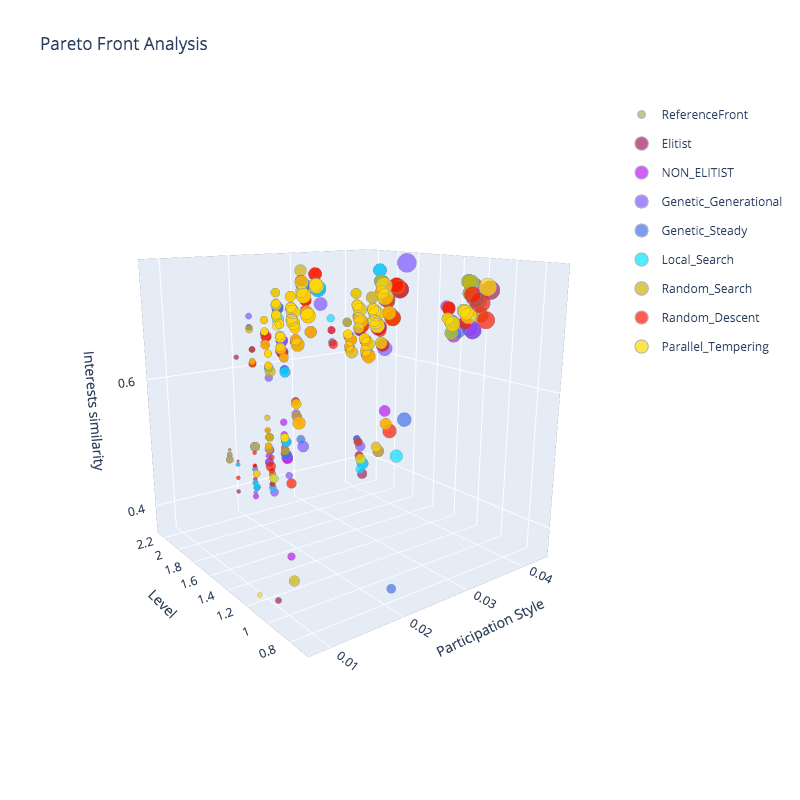
\includegraphics[width=\textwidth]{images/3d_front_mixed_20_soa.png}
    \caption{Caption}
    \label{fig:my_label}
\end{figure}

\begin{figure}
    \centering
    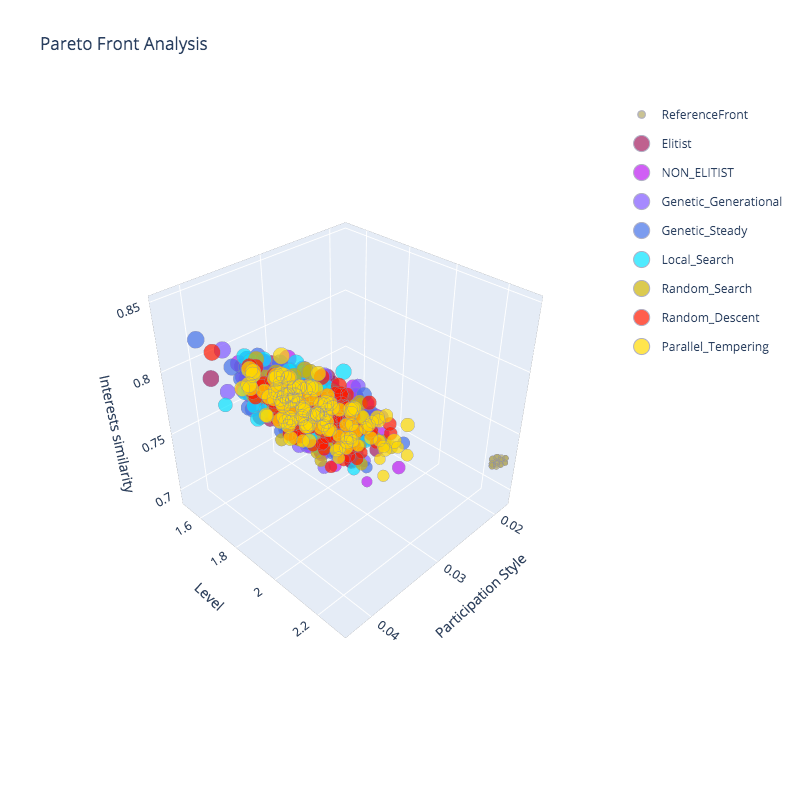
\includegraphics[width=\textwidth]{images/3d_front_mixed_200_soa.png}
    \caption{Caption}
    \label{fig:my_label}
\end{figure}

\begin{figure}
    \centering
    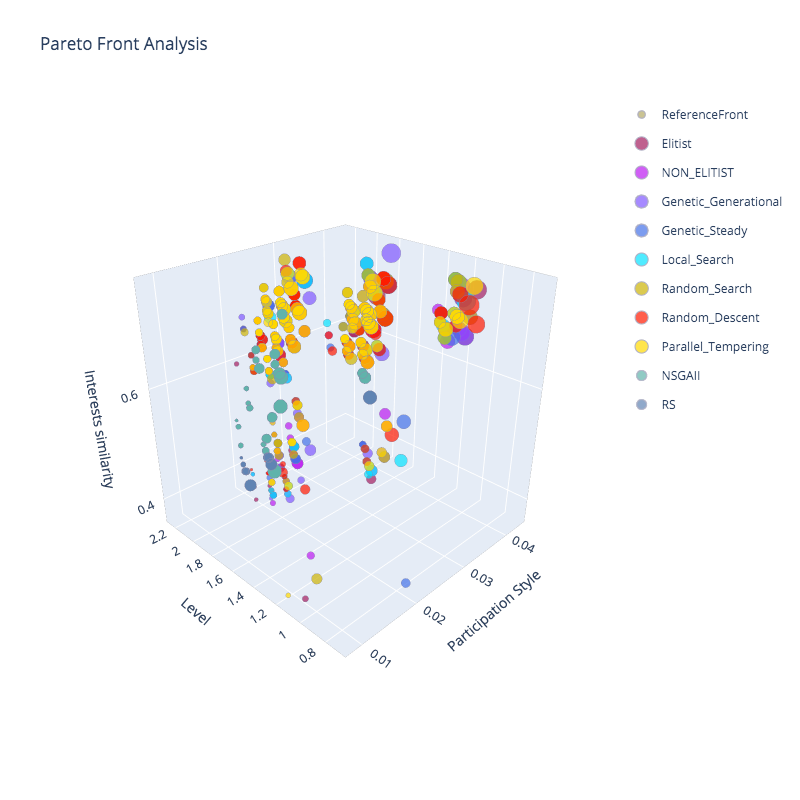
\includegraphics[width=\textwidth]{images/3d_front_mized_20_moa_alt.png}
    \caption{Caption}
    \label{fig:my_label}
\end{figure}

\begin{figure}
    \centering
    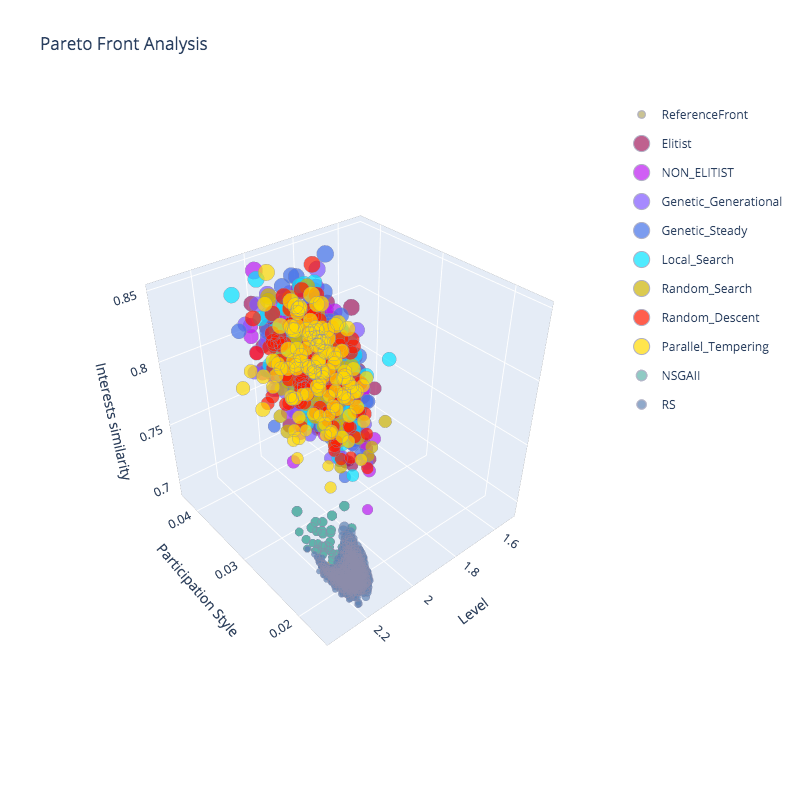
\includegraphics[width=\textwidth]{images/3d_front_mixed_200_moa_alt.png}
    \caption{Caption}
    \label{fig:my_label}
\end{figure}

%-----

\begin{figure}
    \centering
    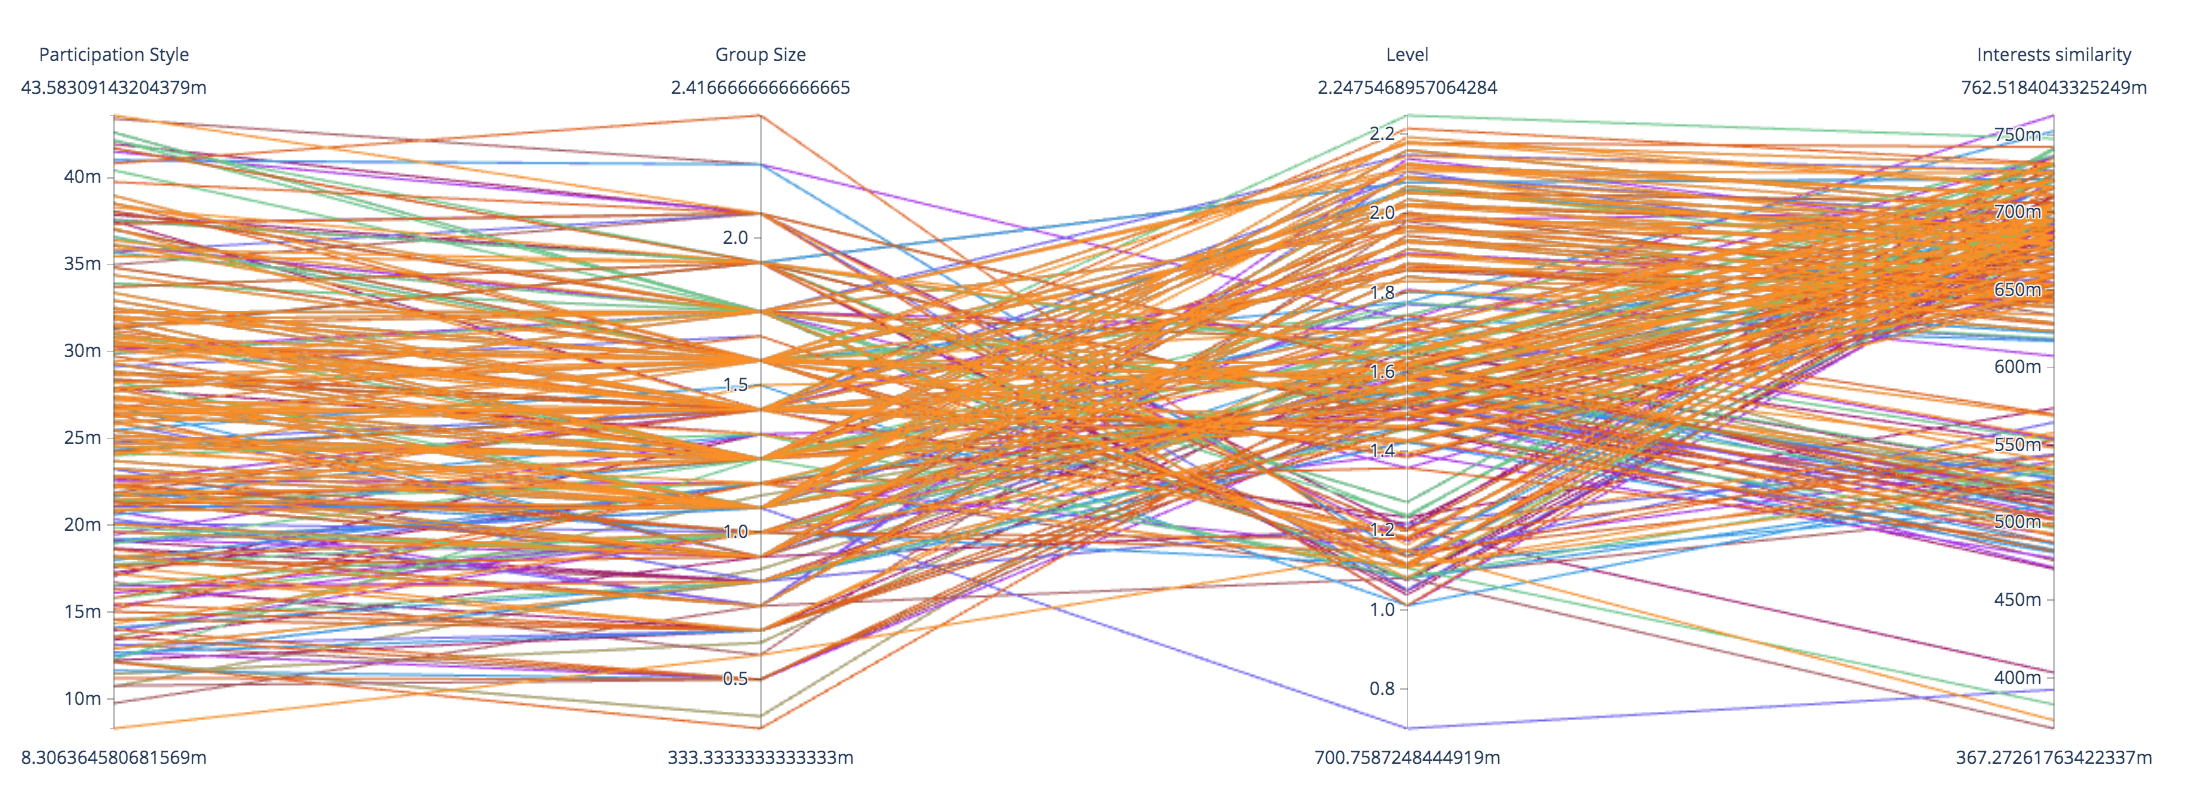
\includegraphics[width=\textwidth]{images/para_front_mixed_20_soa.png}
    \caption{Caption}
    \label{fig:my_label}
\end{figure}

\begin{figure}
    \centering
    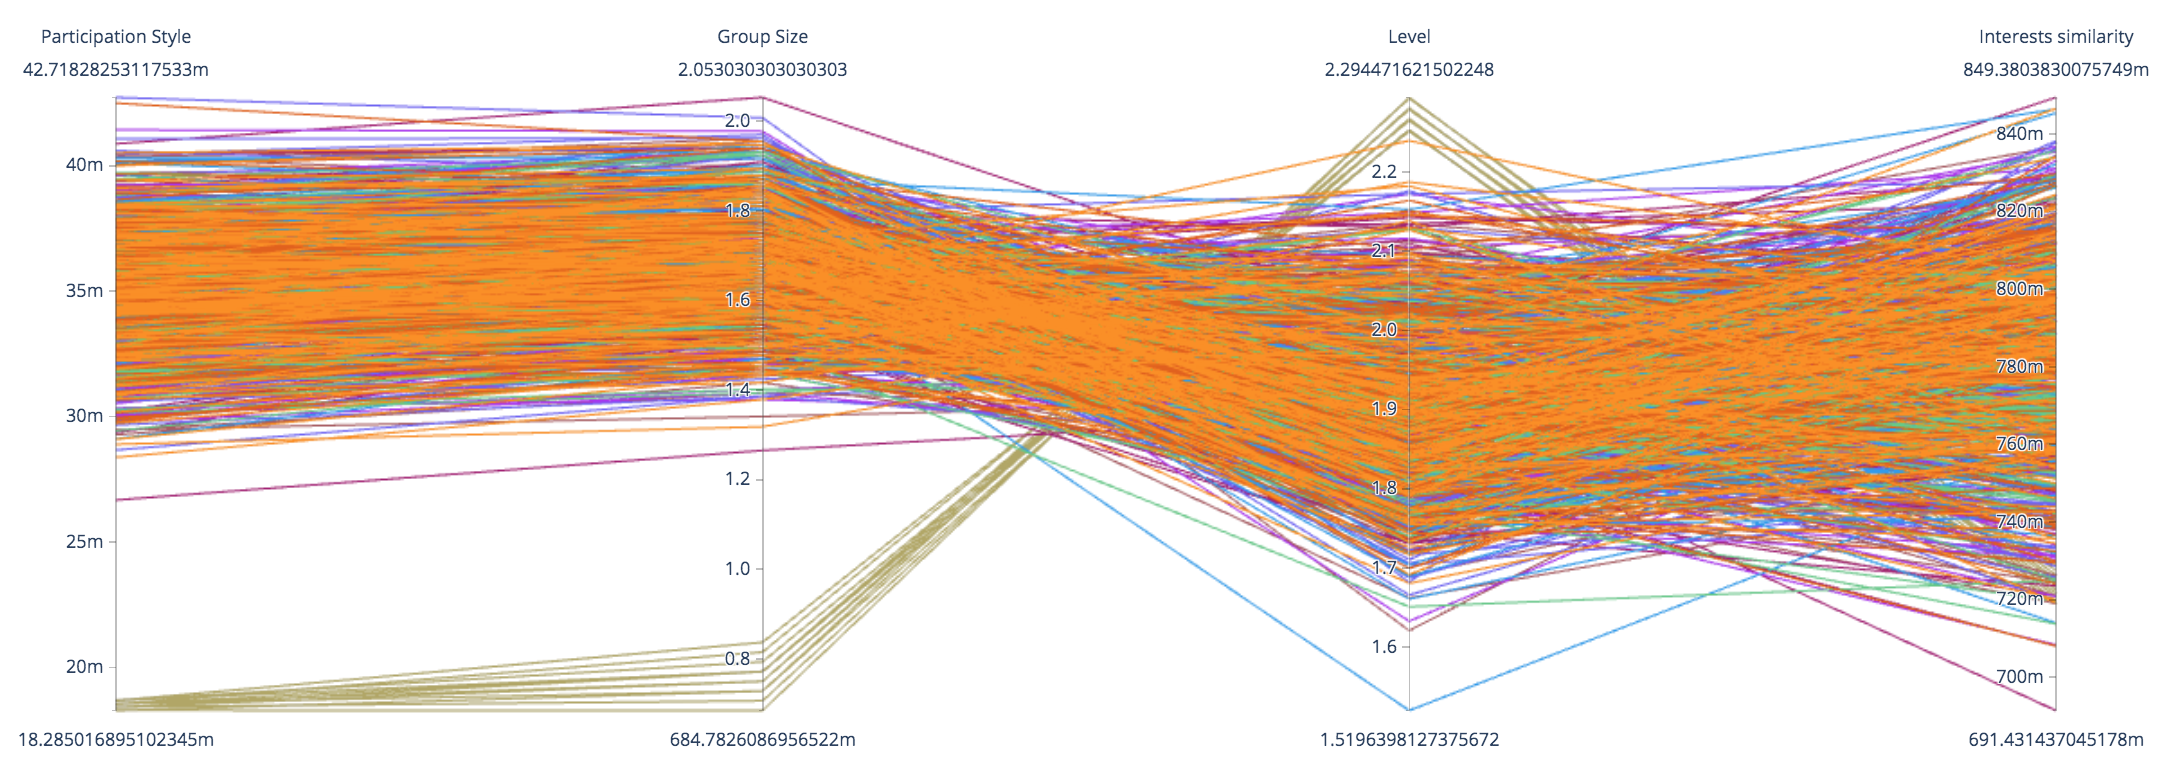
\includegraphics[width=\textwidth]{images/para_front_mixed_200_soa.png}
    \caption{Caption}
    \label{fig:my_label}
\end{figure}

\begin{figure}
    \centering
    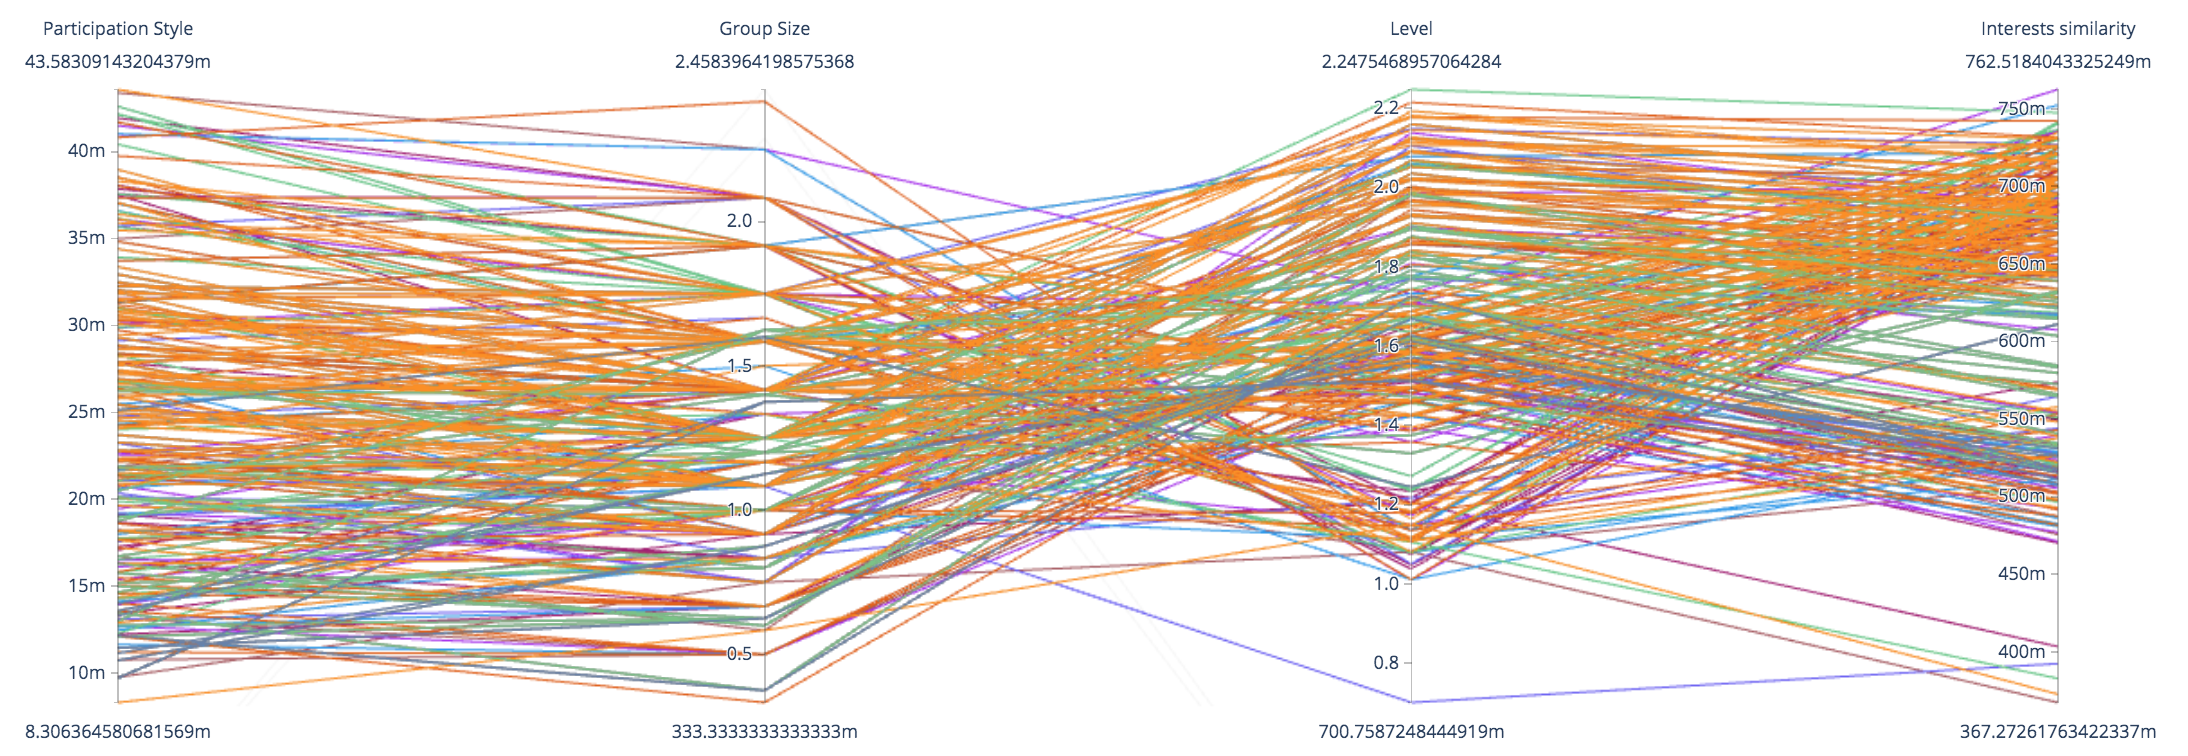
\includegraphics[width=\textwidth]{images/para_front_mixed_20_moa.png}
    \caption{Caption}
    \label{fig:my_label}
\end{figure}

\begin{figure}
    \centering
    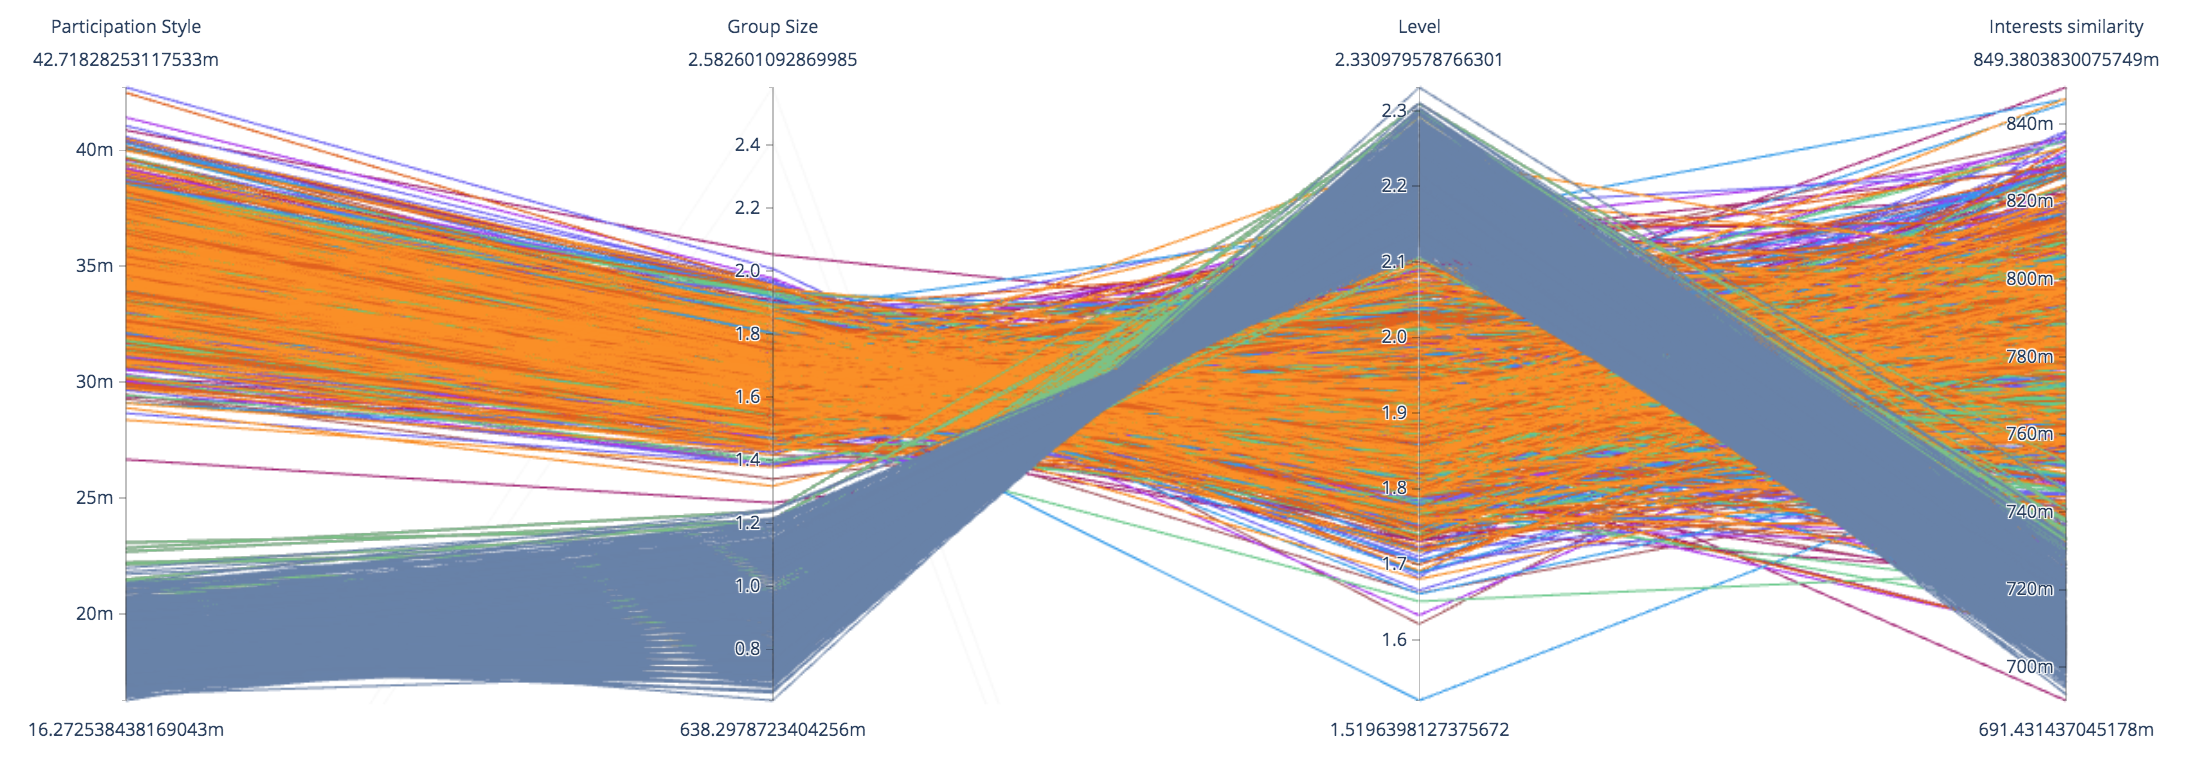
\includegraphics[width=\textwidth]{images/para_front_mized_200_moa.png}
    \caption{Caption}
    \label{fig:my_label}
\end{figure}


% - After the experiments ran, it was noted that even after the pareto front construction none of the algorithms were able to outperform MOAs

\section{Third Phase}

As already established in Phase one and Phase two, $MOA$ outperformed $SOA$ starting from a \textbf{200} size problem, and mostly outperformed them also in the smaller problem of \textbf{20}. However, according to the Friedman test, the algorithm that outperformed all the algorithms overall was $RS$ which meant that no optimisation was taken place, just random solutions outperforming each other. \\

This suggests that there is opportunity for additional parameter tuning. Therefore for this last set of experiments, it was considered only the two other best algorithms from $SOA$ which were $ESPEA$ and $NSGA-II$. These were adjusted according to a set of parameters according to the ones used to obtain best performance for $SMP$ found in \cite{}. Also it was applied a rule of thumb indicating to use \textbf{3} to \textbf{7} times the size of the problem for the population to have a better coverage for the search space \cite{}. Finally, other variations for these algorithms were also tested, using different replacement strategies for $ESPEA$ and different variations of the $NSGA-II$ algorithm. \\

Like the in last phase, these experiments were only tested for the \textbf{20} and \textbf{200} dataset sizes.

\begin{figure}
    \centering
    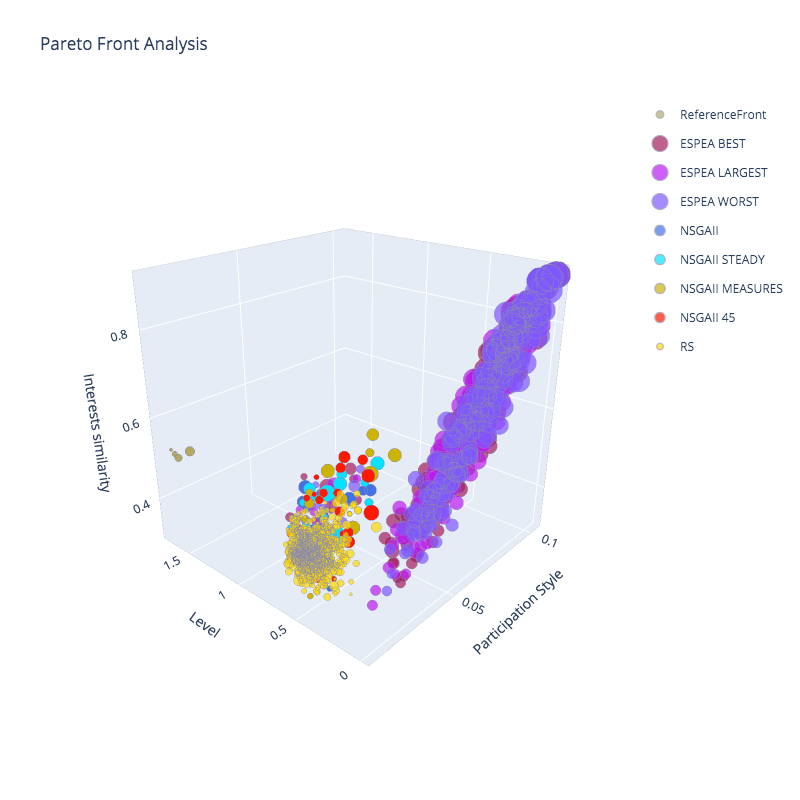
\includegraphics[width=\textwidth]{images/3d_smp_20.png}
    \caption{Caption}
    \label{fig:my_label}
\end{figure}

\begin{figure}
    \centering
    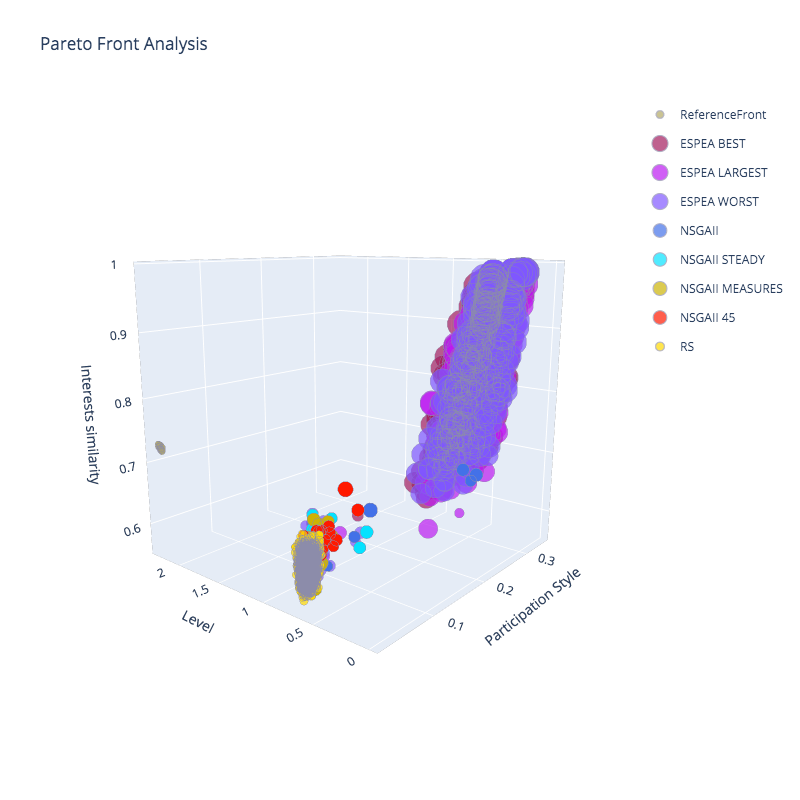
\includegraphics[width=\textwidth]{images/3d_smp_200.png}
    \caption{Caption}
    \label{fig:my_label}
\end{figure}

\begin{figure}
    \centering
    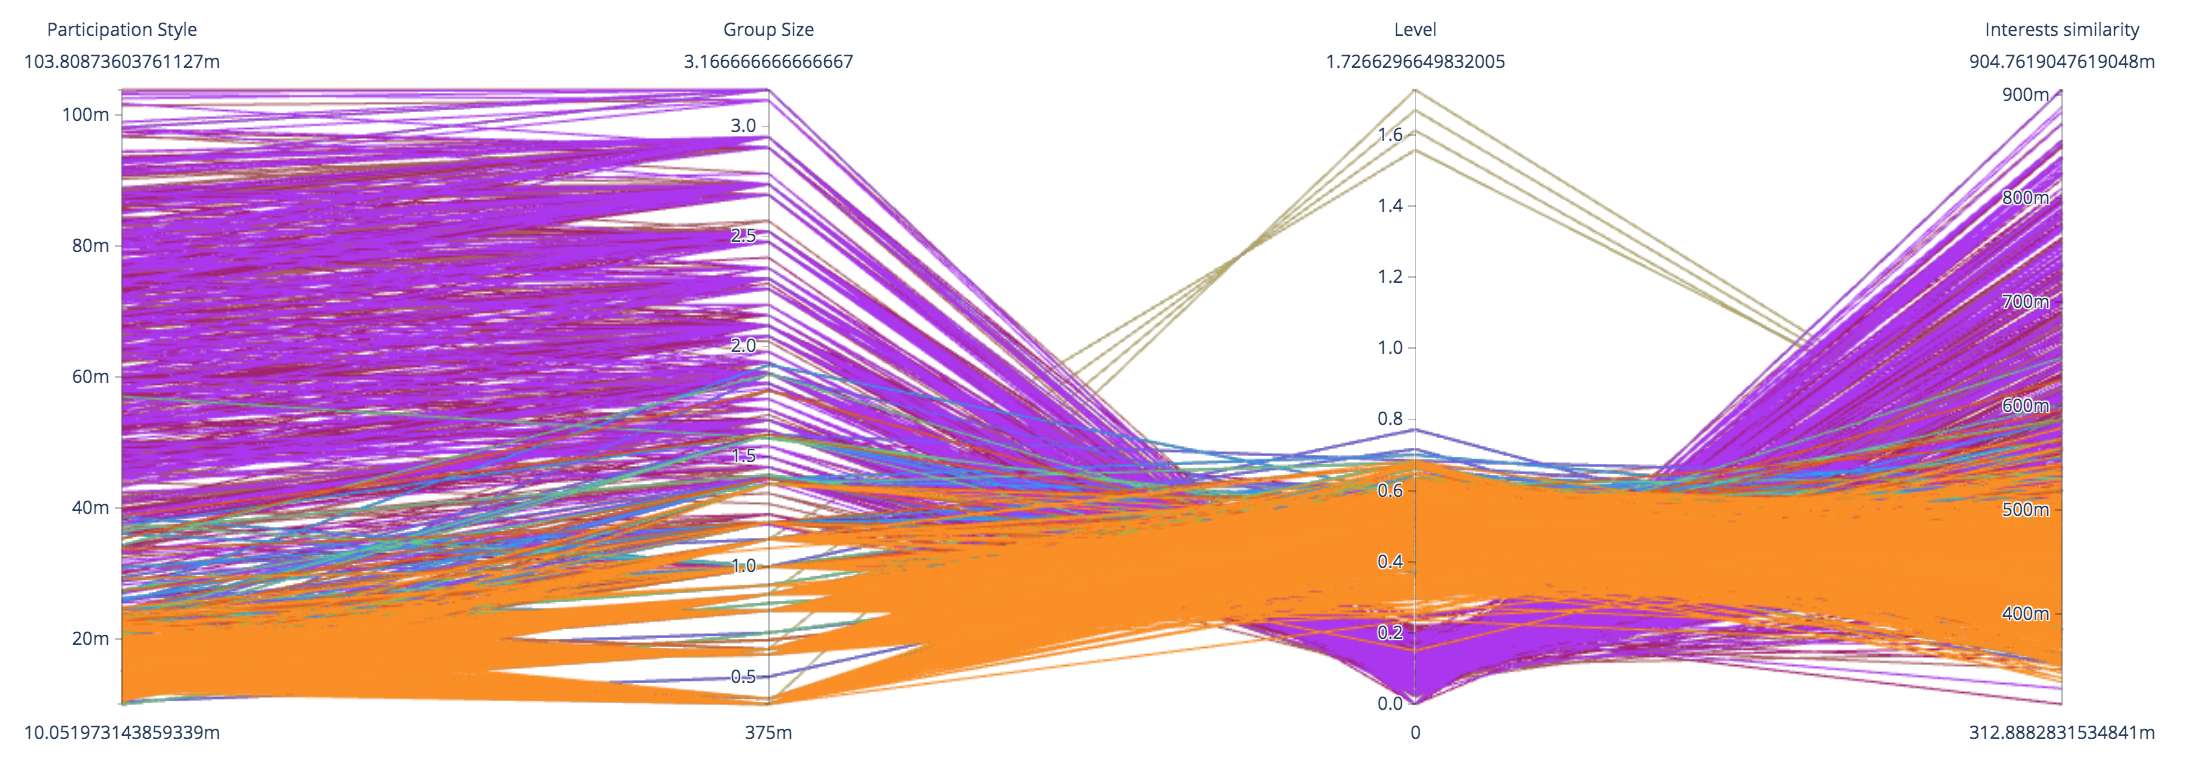
\includegraphics[width=\textwidth]{images/para_smp_20.png}
    \caption{Caption}
    \label{fig:my_label}
\end{figure}

\begin{figure}
    \centering
    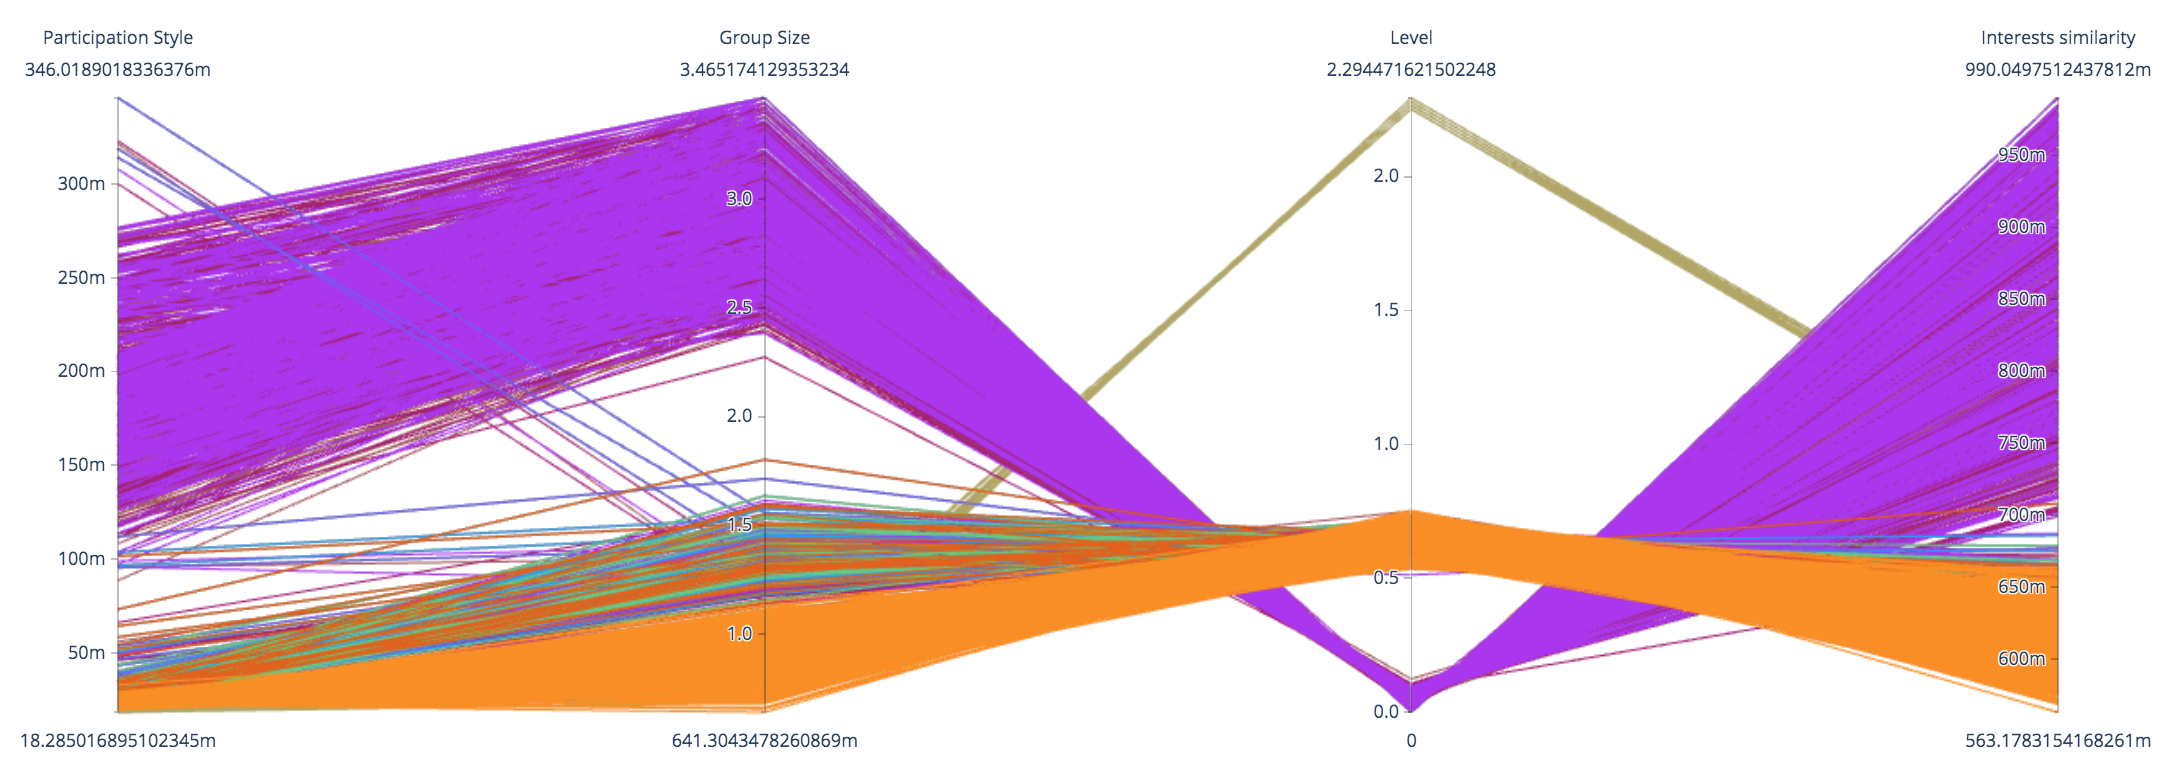
\includegraphics[width=\textwidth]{images/para_smp_200.png}
    \caption{Caption}
    \label{fig:my_label}
\end{figure}


% - NSGAII was finally able to outperform RS using X parameters with an improvement in its Hypervolume.